\documentclass[UTF8]{ctexart}
\usepackage{color}
\usepackage{fancyhdr}
\usepackage[a4paper, left=1in, right=1in, top=1in, bottom=1in]{geometry}
\usepackage{graphicx}

\pagestyle{fancy}
\fancyhf{}
\renewcommand{\headrulewidth}{0pt}
\renewcommand{\footrulewidth}{0pt}
\lhead{杂物版《黑客帝国3:矩阵革命》解读}
\rhead{\thepage}

\definecolor{green}{rgb}{0.0, 0.25, 0.0}
\newcommand{\myparsep}{\noindent \rule[0.5ex]{\linewidth}{1pt}}
\newcommand{\mysection}[1]{\vspace{1ex} {\centering \bf \#1 \par} \vspace{1ex}}
\newenvironment{myquote}{\color{green} \setlength{\leftskip}{6em} \setlength{\rightskip}{4em} \setlength{\parindent}{-2em}}{\par}

\hyphenation{ani-ma-trix}

\begin{document}
\centerline{\bf \fontsize{15.75pt} \baselineskip \selectfont《黑客帝国3:矩阵革命》解读}
\vspace{12pt}
\centerline{作者:杂物}
\centerline{2007-06-07}
\centerline{重制:woctordho}
\centerline{2017-04-01}
\vspace{12pt}

趁热打铁,Neptuneneo刚把第一部重新解读了一遍,我就把第三部的解读发到吧上来吧。现在还没有写完,不是因为neverwin那样的时间关系,只是从那里开始,导演少了些叔本华似的悲观,多了些尼采的期待,我只好开始读尼采的《偶像的黄昏》来恶补一下。另外,这部分写好有一段时间了,文章中的时间和我们现在的时间不符,我就不改了。

看过neverwin达人的两部(一部半,期待他做完第二部)非官方解释,各位应该知道黑迷的看电影方式了,所以我也不废话讲述研究电影内涵的意义。不过我要指出的是:neverwin的作品在一定程度上解答了很多关于黑客帝国本身剧情的问题,但是没能系统的涉及导演所表现的哲学体系。电影中使用的小道具被挖掘出来,并不能证明这部电影的伟大,所以我才耽搁了不少时间,按黑客帝国的内容来学习哲学,以重新看待黑客帝国的意义所在,结果发现完全发掘出黑客帝国的内涵是不现实的,所以我这部作品只不过是《黑客帝国第三部的非官方解释——1》, 以后有了更深的认识必定会有2、3的。

\myparsep

\mysection{写在前面}

对于不了解黑客帝国的人来说,看这篇文章的第一感觉就是我是在把别人的思想往黑客帝国上安,这些都不是导演的本意。但是我要说的是,任何细小的细节都是有其意义的。弗洛伊德在《精神分析引论》中强调人们所做的一切都有其意义,甚至是遗忘什么东西都可以反映一个人的心理。所以我们绝不能无视任何细节,但是细节也有轻重之分,有些只能表现人物心理,有些配合剧情发展,有些解答影片中的问题,有些则体现真理(确切的说,是一种认知)。黑客帝国的出众就在于对于哲学的认知高人一等。

很多电影都试图用这种方式提升自己的档次,可以说有一些效果,但是仍然没有自身的思想。比如,以前有人说《黑暗都市》比黑客帝国内涵高深,于是引起我的兴趣,仔细地看了几遍,结果除了笛卡尔的怀疑论一无所获(指思想方面,其余的符号也是很丰富的,不过就笛卡尔的怀疑论来说,《十三楼》更为出色)。所以说这一套看电影的方式并不适合每一部电影,你若是这样看待每一部电影的话就会失去很多的乐趣。

那些认为自己很聪明的人也不要试图反驳黑客帝国的内涵。哲学家齐泽克曾写了一篇文章说黑客帝国没什么了不起,但是他用康德、尼采的各种理论混乱地解释了一番,并以此作为依据推测后两部的剧情,结果错得一塌糊涂。在没有达到齐泽克大师水平之前,各位天才就本着学习的态度看待黑客帝国吧。

再次引用导演的一句话,黑客帝国有一百层,有些人看到两层就觉得很有趣了,有些人可以看到五十层。我要补充一句:只能看到一层的人,不要开口说黑客帝国只有一层。

\myparsep

\vspace*{\fill}
\mysection{正文开始}
\vspace*{\fill}

\newpage

经典的Matrix开头,很多人称此为数字流,但是我们应该看到这些流动的符号很多是日文假名,还有希腊字母,还有剧组造出来的符号,导演俩在后两部的原版剧本里曾经提到Matrix并非二进制的电脑(虽然电影中有个人物叫做Binary)。

我们应该思考一个问题,二进制是否可以成为真正的智能?neverwin曾在第一部的非官方解释中提到一种哲学的认知方式,在多项选择中,我们可以看其为选项1和非选项1,也就是把除了选项1的所有选项看作一个整体。当然这只是一种认知方式,而且是我们基本无法掌握的认知方式。如果Matrix是类人逻辑的AI所造,那我们也必然要抛弃简单二进制智能的说法。在我看来,人类和机器的智能区别就在于社会结构的不同。

\begin{figure}[htb]
\centering
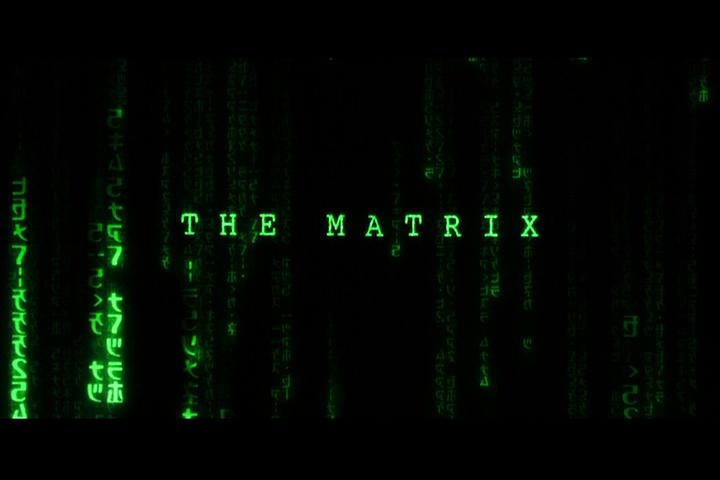
\includegraphics[width=0.5\linewidth]{fig/eeeb9f515ea2062442a75b17.jpg}
\end{figure}

题目的后半部分是Revolutions. 不光是革命,还是复数。有必要理解一下这个复数所代表的多重革命:

1、自由人类对Matrix非选择性工作体制的革命。

2、无目的程序对Matrix删除制度的革命。

3、过期程序对Matrix强行安排固有命运的革命。

4、人类内部对于Matrix性质认识的革命。

每一种都会在后面详细解释,这里就不多讲了,其实在这里也讲不出什么实质来。

\begin{figure}[htb]
\centering
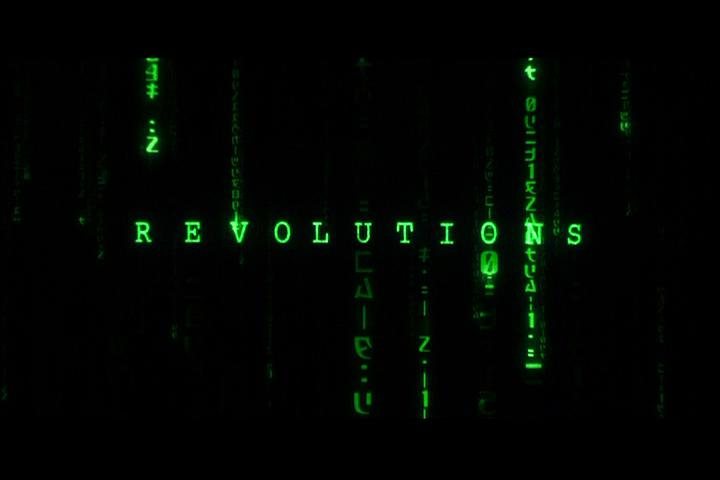
\includegraphics[width=0.5\linewidth]{fig/0b330eb35d354ba7d9335a17.jpg}
\end{figure}

金色,灵魂的颜色。哲学家音轨里两位教授都是这么认为的。金色的爆炸就意味着灵魂的诞生和飞速发展。从电影看来,金色是特指机器的灵魂,人类则缺少这么灿烂的光芒。Neo在瞎了眼之后可以感觉到被人类视为仇敌的机器,却看不到自己的另一半Trinity,就是最好的证明。

\begin{figure}[htb]
\centering

\includegraphics[width=0.5\linewidth]{fig/9ad10e2411b6d033c8955917.jpg}
\end{figure}

吧友一杯冰牛奶曾经指出这是数学中的分形结构,也具体指出了是哪一种,我认为哪一种不重要,而是分形所表达的意思。分形结构对于没有接触过这个方面的人(我就对分形一无所知)来说,最大的特点就是自我中有自我,生生不息。你可以从这个图形的任何一部分中找出这个图形本身。就像两面正对着的镜子,你可以从任何一面镜子(包括镜子的像)中找出其余任何一面镜子的像。于是我认为这里导演想要表达的意思就是,机器在发展的过程中不断地产生自我,完善自我。虽然更为精致、更为智慧,但这是一再重复着的、没有本质变化的进化。

\begin{figure}[htb]
\centering
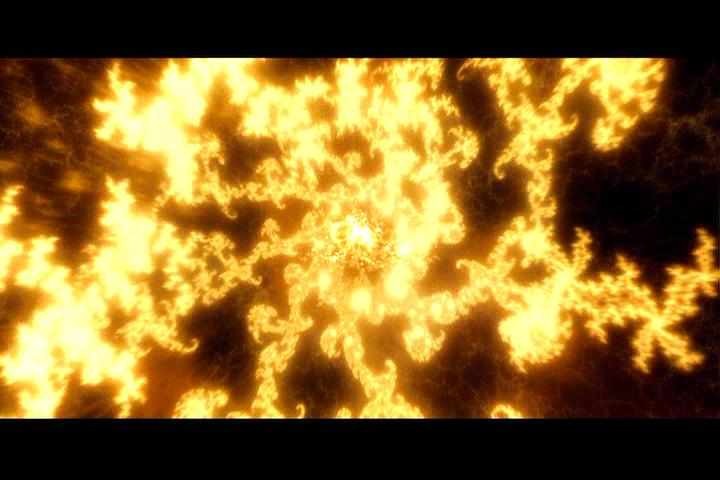
\includegraphics[width=0.5\linewidth]{fig/84bda8ec1f016a2762d09f11.jpg}
\end{figure}

这就是机器城啊!Neo在Logos号向下俯冲的时候看到的就是这个景象。从这以后,前伸的镜头开始倒退,我们看到的就不再是机器灵魂的灿烂金光,而是Matrix的代码。如果说第三部的开头代表的是AI的成长,这里无疑意味着“第二次文艺复兴”(the Second Renaissance),机器建立了机器城,和人类打了一仗,然后就靠着Matrix安逸地生存。

\begin{figure}[htb]
\centering
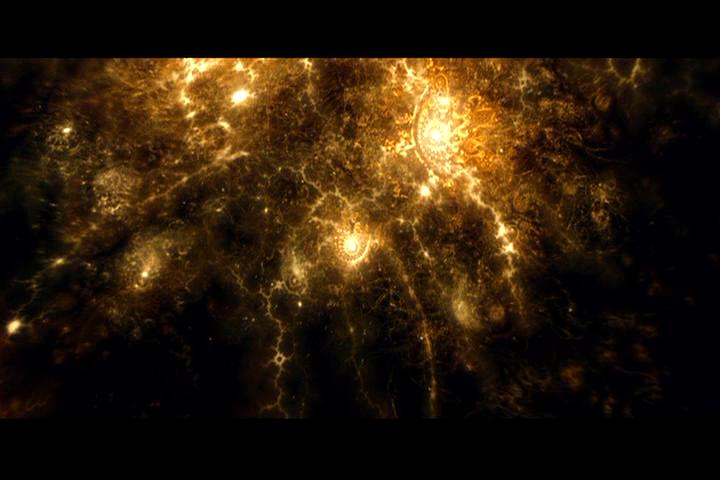
\includegraphics[width=0.5\linewidth]{fig/3c8e8b13f5356bd0f7039e11.jpg}
\end{figure}

这里就是人类历史上的最大转折点“第二次文艺复兴”。之后,绝大部分人类生活的世界。我要指出的是,这个世界没有机器的外在压迫,人类要对抗机器的唯一正当理由就是为了Zion25万居民的生存,还有就是对Matrix内部人类社会发展的限制。这限制就是:二十世纪初人类发明AI,AI发展到和人类对抗的地步,人类战败后在Matrix里度过了大约6个世纪(前两个失败版本还未计算进去),所以外在世界至少是26世纪了。即便是Morpheus所说的22世纪,Matrix也已经对人类自然发展造成了一个巨大的障碍。不过这不应该是我们要把机器干尽杀绝的理由,罗素在《西方哲学史》中说亚里士多德延缓了科学的发展,但是他仍然把亚里士多德当作大哲学家,大科学家。同理,机器也不该因此被称作奴隶主。况且,科学是双刃剑,任由人类自由的飞速发展,还不知道我们是否能活到26世纪呢。

当然,这种“自由”的概念是黑客帝国官方网站上写论文的那些哲学家的思想,也是大多数人接受的“自由”概念。导演要表现的却是叔本华所说的绝对自由,也就是第三种自由,不光是“我能做我想做的”,而是“我要不受限制、随意地做我想做的”。这句话非常难表达,我这么说其实已经陷入了叔本华所说的循环中。要完全理解这第三种自由,还是看看叔本华本人《悲观论卷集》中在《伦理学的两个基本问题》里对概念的规定。这里我只能这么说:“绝对自由是无序的,不可预测的。”这个理论会在后面由Smith指出。

\begin{figure}[htb]
\centering
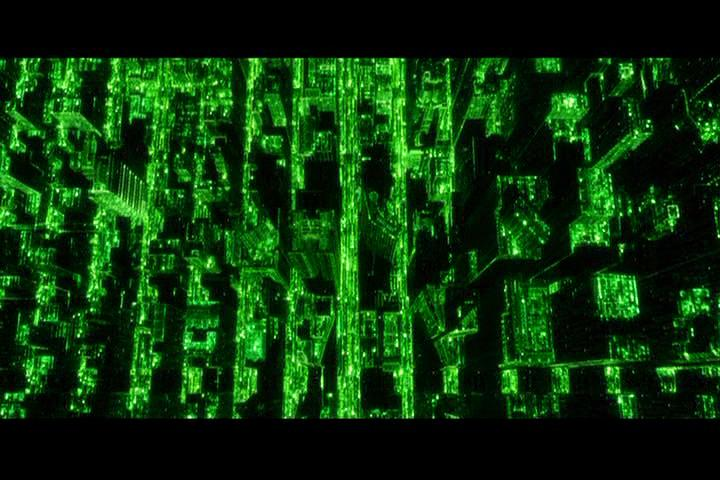
\includegraphics[width=0.5\linewidth]{fig/1f716227f5c2fe03918f9d11.jpg}
\end{figure}

这个图形非常有趣。要知道导演Wachowski兄弟(也许是姐弟了)来自芝加哥,酷爱篮球,偶象是飞人乔丹,最喜欢的篮球队就是芝加哥公牛队。几乎在每个国外的黑迷论坛上都提到这个图形的来历,那就是芝加哥公牛队的标志。同时,导演俩还把Mega City设计为这个标志的形状。无论是第二部的高速公路还是最后Neo和Smith决战的大街,都设计在了这张地图上。这也看出了导演俩对于符号的热爱。(导演俩在拍电影前搞了多年的漫画,漫画是最崇尚符号使用的。现在两人拥有一家漫画公司Burly Man Entertainment,Burly Man就是当初拍摄黑客帝国时用的替代名)

\begin{figure}[htb]
\centering
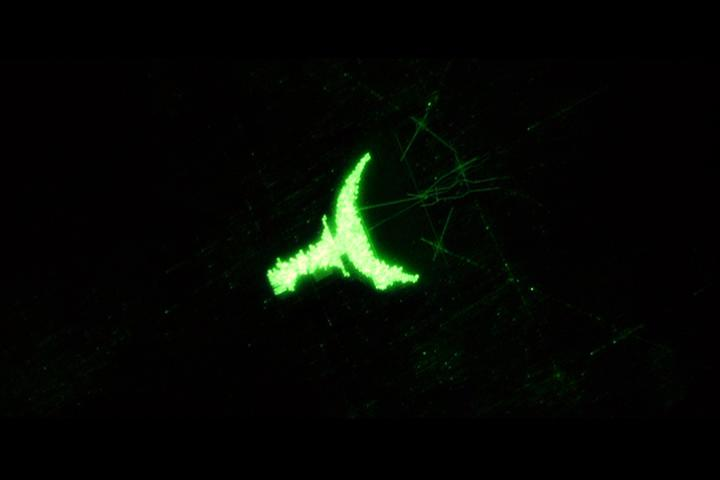
\includegraphics[width=0.5\linewidth]{fig/245732fa9999af1ea8d31110.jpg}
\end{figure}

Matrix在屏幕中,屏幕的意象是明白到不能再明白的了。屏幕中的就是拟像,还要再提一下已经被我们引用过成千上万遍的鲍德里亚的名言:“拟像不能使我们想象现实的存在,而本身就是虚拟存在的真实。”这里有必要提一下《十三楼》,在黑客帝国两个月后上映实在是太可怜了,本身也是一部很好的作品啊。除了结尾以外,对笛卡尔的“我思故我在”解释是很精辟的。

这里提出来说呢,是因为《十三楼》中的虚拟世界里,连人类都是完全虚拟的。这就更有针对性了,电影中把这些虚拟人也认作是人,和鲍德里亚所表达的意思一致。不过黑客帝国对鲍德里亚哲学解析的精髓不在这里,而在第一部中Cypher和Trinity的对话中。导演使用他的“虚拟现实”化解了昂格尔(Peter Unger)的“真实的价值”(Value of the Truth)对诺齐克(Robert Nozick)“经验机器”(The experience machine)的攻击。到第三部,导演就不再对“虚拟现实”进行更深入的解析,不过符号的拿手戏还是没有放下。

\begin{figure}[htb]
\centering
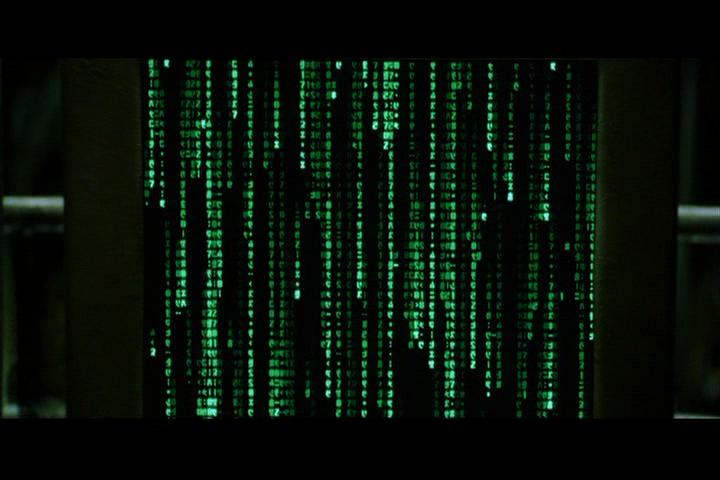
\includegraphics[width=0.5\linewidth]{fig/a698838bba0ca1d3fd1f1010.jpg}
\end{figure}

\begin{myquote}
AK: I got nothing, sir. No sign of Niobe or Ghost. Nothin' but blue pills.

Mauser: Should we jack in and try to contact them?

Roland: It wouldn't matter. My gut says they're down.

Mauser: Then we should start back.

Roland: No. If that ship can still fly, then we need it.

Mauser: I was afraid you were gonna say that.
\end{myquote}

这里解释一下他们的话,那句blue pill就是指代有机会出来但没有出来的人,他们没有勇气接受现实的改变,就和机器一样。其实大多数人都是如此,搞不好我就是一个blue pill。

Roland说:“只要那艘船还能飞,我们就需要它。”其实他们需要的是Logos的EMP。这里要说一下,EMP是装在飞船上,拿不下来的。而且根据每艘船的铭牌,这些船都是机器城制造的,所以说人类没有能力制造更多的EMP来对抗机器。而且电影里的EMP和我们现在不同,我们现在都已经有能力对付EMP了。说EMP和现代的不同还有另一个原因,《第二次文艺复兴》中,人类对机器使用核弹但是收效甚微,核弹爆炸也会产生EMP的效果,足以说明当时的机器就有能力对抗EMP了。机器造这些新式EMP给人类来攻击自己的目的会在后面解释。而Zion城其实也是机器留给人类的,是上一代救世主救出23个人之后就把他们带到Zion,以前也有Fan Fiction说Zion是以前的人类军事基地。所以说Zion的来历并不重要,我们有足够的理由认为Zion存在着。

\begin{figure}[htb]
\centering
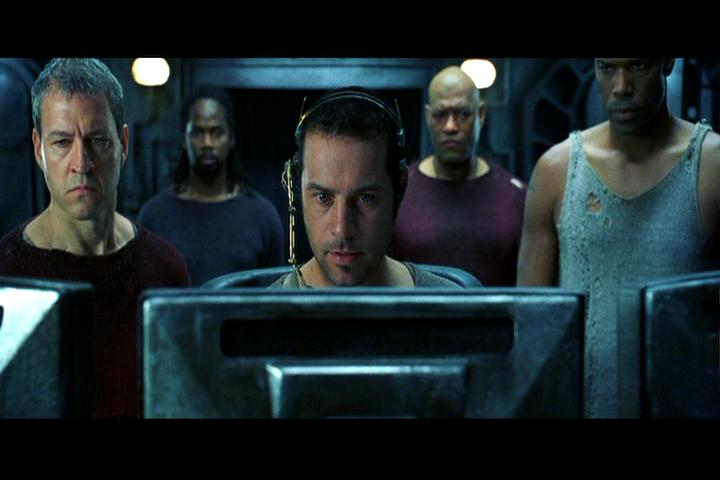
\includegraphics[width=0.5\linewidth]{fig/17e9a71eb5c1f41f41341710.jpg}
\end{figure}

\begin{myquote}
Roland: Search every pipe, every hole, every crack we know. Sweep as wide as possible, as fast as possible.

AK: Captain, these lines are crawling with calamari.

Roland: Then the sooner we find them the better.
\end{myquote}

现在说一下这些人的名字:

船长Roland, 这个名字可能源于查理曼大帝的法兰克管家。在史蒂芬金的作品The Dark Tower中,他被形容为一个枪手。而他的手下正好都以武器为名字。

大副Colt, 柯尔特自动手枪,喜欢枪械的朋友一定不会陌生。

接线员AK, 连对武器一窍不通的人都应该听说过著名的AK47。

船员Mauser, 德国毛瑟枪,简陋而原始的枪,用黑人来演自然是表示原始的力量。

医护员Maggie, 是Margaret的缩写,那是一本著名的关于枪械武器的杂志。

\begin{figure}[htb]
\centering
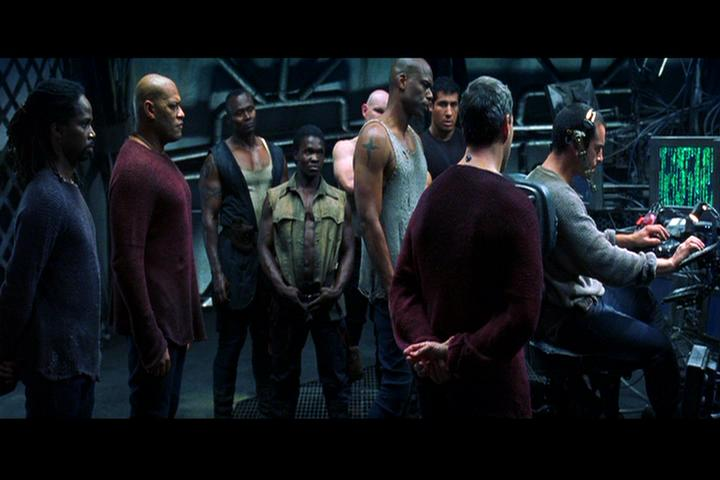
\includegraphics[width=0.5\linewidth]{fig/84bda8ec1f006a2762d09f12.jpg}
\end{figure}

\begin{myquote}
Maggie: Thought you could use something to eat.

Trinity: Thank you.

Maggie: Any change?

Trinity: No. How's he?

Maggie: He's going to be fine, at least until he wakes up.

Trinity: What do you mean?

Maggie: The captain has some questions for him. He better have some good answers. You see these cuts? I think they're self-inflicted.

Trinity: Why?

Maggie: VDTs, maybe. I don't know. But like I said, the answer had better be good.
\end{myquote}

我在第一次看这部电影的时候,没有去查这个VDT的意思,想当然的认为VDT是精神分裂之类的病症。仔细查了之后才知道这是导演兄弟自己编出来的词汇,意思是virtual delirium tremens,虚拟震颠性谵妄。本来是有delirium tremens这个医学名词的,其最明显的症状就是“幻觉”。

在这部片子的评论音轨(哲学家音轨)中,Ken Wilber和Cornel West都提出这第三部是三部曲的循环部分,连接部分。第二部在这里结束,第三部就在这里开始。而且导演俩也比前两部更注重平衡和阴阳,以尽可能和谐的构图来表现这部电影,画面非常对称,对单个人物的特写全都构建在镜头的半面,几乎是完美的平分画面。这一点在导演俩的处女作《Bound》里就做得非常出色。

这里既然出现了Trinity, 那就再谈一谈Trinity和the One的关系。trinity的拉丁文变体为tria iuncta in uno,那就是三溶于一。先知说过尼奥之路是由众人组成的,Trinity就是最重要的部分。Ken Wilber和West博士都在音轨里说过,没有Trinity的the One是不完整的。

\begin{figure}[htb]
\centering
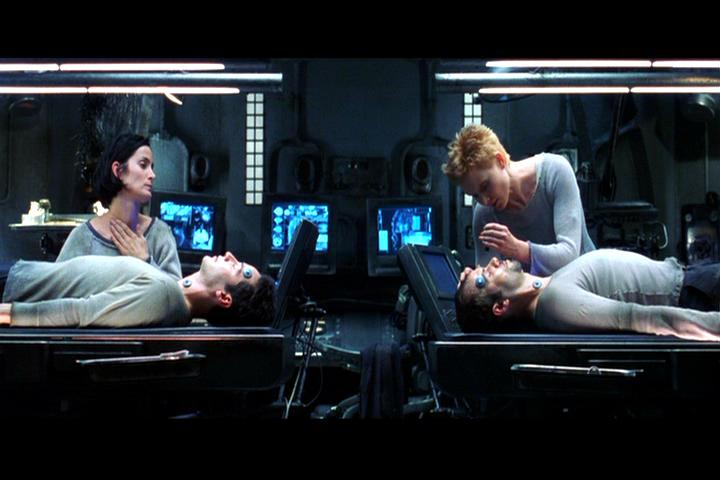
\includegraphics[width=0.5\linewidth]{fig/3c8e8b13f5346bd0f7039e12.jpg}
\end{figure}

\begin{myquote}
Morpheus: Roland. I'd like to run another search through the Matrix.

Roland: For what?

Morpheus: For Neo.

AK: How can he be in the Matrix, sir? He's not plugged in.

Morpheus: Please, for me.
\end{myquote}

Morpheus不愧是梦神,一下就明白了Neo的精神到了另一个世界。但是我们要注意的是,Neo的精神和身体并未分离,即便Neo到了另一个世界,他还有一个“自我形象”可以控制。正如世界本质的几个假说造物说、计算说等等,无论你身体的本质如何改变,这始终是你的身体。

\begin{myquote}
Maggie: This is what keeps bothering me.

Trinity: What?

Maggie: His neural patterns don't read like someone who's in a coma. The strange thing is, I see these patterns all the time.

Trinity: Where?

Maggie: On someone jacked in.
\end{myquote}

本来Morpheus这么一说,外加Maggie这么一补充,我们都会以为Neo就在Matrix中,导演却安排AK这么回答:

\begin{myquote}
AK: The big bubkis. Nada. He's not in there.

Colt: Sir, we've got the projections!

Roland: How long?

Colt: Based on the point of entry and the [past] speed it looks like the machines will be inside of Zion in just under 20 hours.

AK: Jesus H. Christ.

Roland: All right, let's move with a purpose. AK, get upstairs, I want you on holographics. [Colt,] Mauser, I want forward and aft guns manned at all times. And make sure we are running on as few pads as possible.

Colt: Yes, sir.

Link: Hey. Hey! We got a call. Operator. It's Seraph.

Seraph: I bring word from the Oracle. You must come at once.
\end{myquote}

我们敬爱的同胞Seraph出现了,做事雷厉风行,一句话就挂电话。程序的目的啊,不让他废话一句,看来他受着无尽的限制。但没有了规则,程序还能存在吗?我们在这里要回忆一下Seraph的程序目的,“保护最重要的”, 然后再看他接下来的行动吧,就会明白Matrix现在最重要的是什么。

\begin{figure}[htb]
\centering
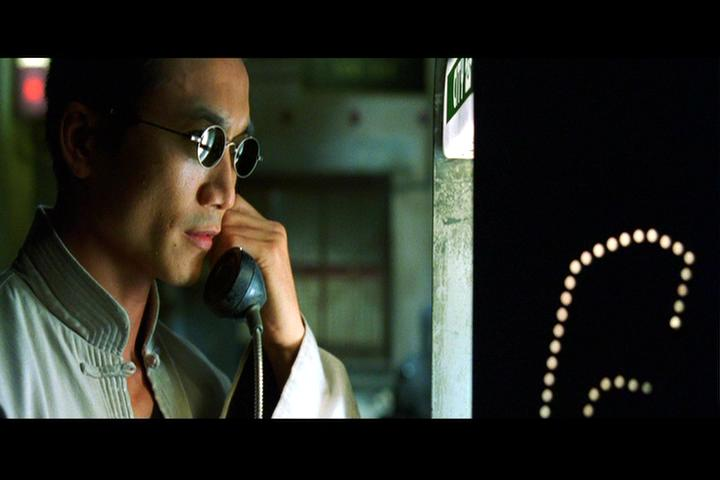
\includegraphics[width=0.5\linewidth]{fig/1f716227f5c3fe03918f9d12.jpg}
\end{figure}

\begin{myquote}
Sati: Good morning.

Neo: Who are you?

Sati: My name is Sati. Your name is Neo. My papa says you're not supposed to be here. He says you must be lost. Are you lost, Neo?

Neo: Where am I?

Sati: This is the train station.

Neo: This isn't the Matrix?

Sati: That's where the train goes. That's where we're going. But you cannot go with us.

Neo: Why not?

Sati: He won't let you.

Neo: Who won't let me?

Sati: The Trainman. *whispers* I don't like him, but my papa says we have to do what the Trainman says, or he will leave us here for ever and ever.
\end{myquote}

揣摩一下这里的话吧,有人指出过Sati这里说的“早上好”很有意思。这里有时间吗?有时间的话,为什么是早上呢?接着,Sati就明白的说出Neo是谁,又是一个疑点。看看这张图,她身边一圈光环。再看一下Sati这个名字吧,是指印度教妻子殉夫的传统,充满祭祀、牺牲的意思。还有一个意思是梵语的“Being”,就是本质、存在、生命这些意思。而且Sati还是印度教的一个神。

叔本华、尼采都是很崇尚印度教的。导演俩也是如此,他们原本在George设计的飞船中起了些Vishnu、Brahma这样的名字。

据说梵天产生此世界,是由于某种错误而成的。为了补偿自己的过失,它便置身于这个世界之中,一直到设法能补偿了为止。如此说明了万物的起源,是多么值得称道!依照佛教的教义,世界的产生,是由于一些莫名其妙的骚扰,打破了涅盘天地的神圣的宁静。

我这里引用一句拉丁谚语:Prudens futuri temporis exitum caliginosa nocte premit Deus.(智慧的神用黑暗卷起未来)

所以导演一直给我们传达一个信息:信仰单一真神,信仰那完美的力量,就是一种逃避。

\begin{figure}[htb]
\centering
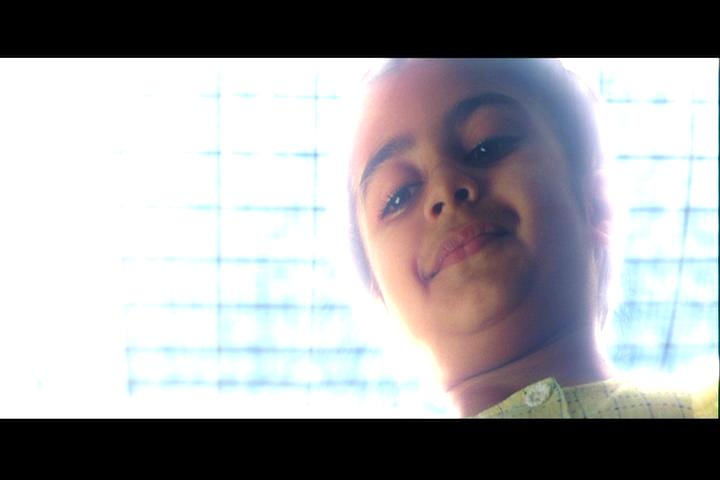
\includegraphics[width=0.5\linewidth]{fig/cce0b3b70bb105f431add112.jpg}
\end{figure}

这里还要注意一句台词,leave us here for ever and ever。没有用Forever, 而是for ever and ever,导演还特别让Sati突出了这部分。这又是一语双关(为什么要用“又”呢?因为neverwin达人在前两部里解释了很多一语双关的例子),意思就是:“你被留在这里是因为过去的事。”比较了解黑客帝国的朋友应该明白这和法国人是什么关系。我们知道法国人掌控Matrix的信息,并以因果律(并非霍金所说的纯物理因果律,这一点会在后面提到)推测过去发生了什么。所以我们每次遇到法国人,他都会准确无误的知道我们来的目的,甚至是一点细节。比如后面我们会看到,法国人一看到Seraph来了就说先知一定找到了新的躯壳。这里法国人就是为了“过去的事”把Neo囚禁了,是哪一件事我们很清楚,呵呵,几分钟就把法国人好不容易培植出的势力干掉了,他能不生气嘛。

另外再说一下Sati的身份,很多人认为Sati是下一代先知。我认为这似是而非,一来Sati是无目的程序,把她分类本来就不对;二来Sati确实有先知的能力。后面我们会看到,Trainman根本不认识Neo, 而Sati却已经知道Trainman不会让Neo走了。我们暂且说Sati是一个有先知能力(还有其他能力,像是控制天气)的无目的程序。

注意这张图中这个火车站的名字,Mobil Ave, 这个Mobil就是Limbo的乱序词。Limbo的意思就是世界间的世界。在但丁的神曲中,Limbo被描述为九层地狱的第一层,里面的人不受折磨,享有无尽的空虚。不相信神,也不反对神的人就会待在这样的地方。而在Matrix中,我们明白,既不相信神也不反对神的人是真正理解神的人、知道神的立场的人。

\begin{figure}[htb]
\centering
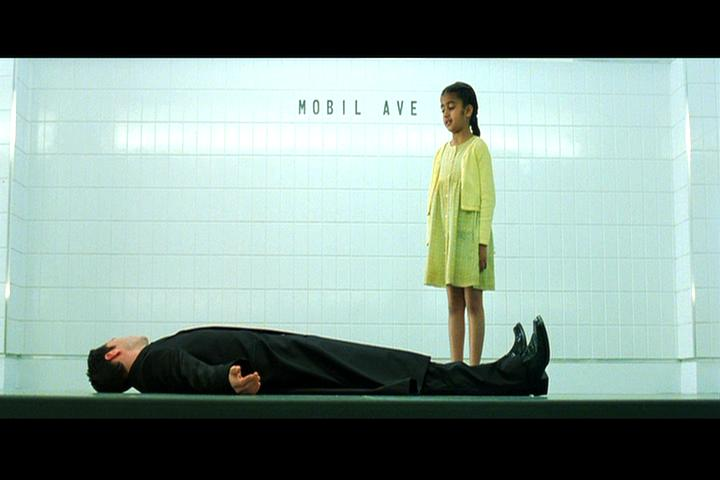
\includegraphics[width=0.5\linewidth]{fig/e36b4a3679b53bdda3cc2b19.jpg}
\end{figure}

\myparsep

马上就要去见先知了。先看看先知公寓那里的情况,看看墙上的涂鸦(可以在黑客帝国官方网站的Zion Archives找到),下面那张图中写的是guts。记得前面Roland说了什么吗?他说:“My gut says they're down.”这一点秉承了叔本华的直觉主义,在先知这里也不例外。我们常说先知的能力可以用因果律、全定论来解释,而叔本华最讨厌的黑格尔也认为“时间是我们看不全面而产生的幻觉”,但是这样一来就无法解释先知只能“believe”未来的相关台词。导演就暗示我们,这不是完美的因果律和全定论,也不是令人不愉快的宿命论,而是我们的直觉。

这一点我之所以不在Roland那里就指出,是为了避免大家误会Roland是直觉主义,而先知是全定论,其实二者都是基于直觉主义的。当然,长期研究人类情感的先知要可靠得多。

\begin{figure}[htb]
\centering
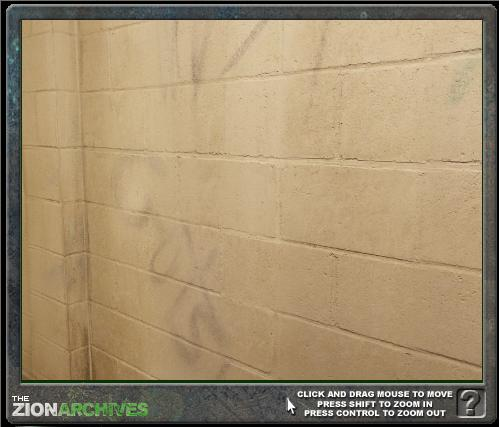
\includegraphics[width=0.5\linewidth]{fig/43ead53fab4bbcc27c1e7125.jpg}
\end{figure}

看一些墙上的涂鸦,这些不像guts这样重要,不过仔细看还是很有趣的。这张没有什么隐藏的意思,就是peace。我们知道先知要的就是peace,先知believe的就是peace。

\begin{figure}[htb]
\centering
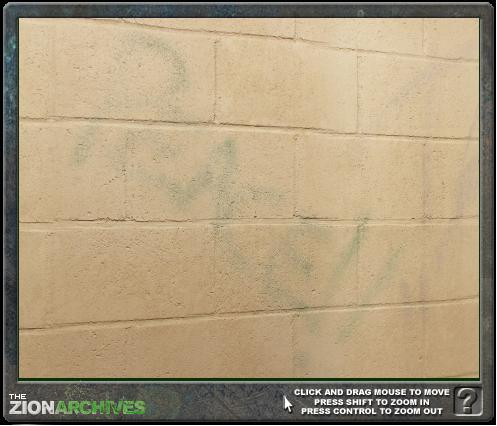
\includegraphics[width=0.5\linewidth]{fig/27d5d1a2c52f2dadcaefd05a.jpg}
\end{figure}

下图上方的图形就是无政府主义的标志,A外一个圆圈,其实V for Vendetta的标志就是从这个标志来的。

\begin{figure}[htb]
\centering
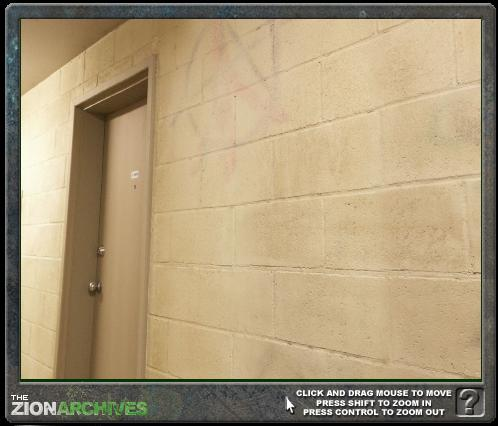
\includegraphics[width=0.5\linewidth]{fig/45c00df4fb76d7ef7709d75a.jpg}
\end{figure}

估计写到这里就已经有人认为我找得过头了。就拿guts来说,有人会问:“这么重要的标志会藏的这么隐晦?”这么说吧,对于一般的观众来说,先知预知未来的能力是不必解释的,这个标志自然就不重要了。但是对于我们这种试图分辨先知是全定论还是直觉主义的人来说,这个标志也不如Neb飞船的铭牌寓意对于虔诚的基督徒来说更隐晦。

整个《黑客帝国》系列,正如叔本华称自己作品“不是写给老百姓看的”一样,不是给普通的影迷或是影评人看的。喜欢《黑客帝国》的哲学家们也不愿意更多的人喜欢《黑客帝国》,因为他们认为只看特技的人不配喜欢《黑客帝国》, 以至于用过于复杂的理论来讨论黑客帝国。一个例子就是哲学家David J. Chalmer甚至在一篇讨论《黑客帝国》的形而上学理论的文章里生造了一个有关存在主义的哲学术语“Envatted”(非原存在,虚拟之类的意思,类似缸中之脑的处境,字典上是查不到这个词的)。在那之后,很多哲学家受他的影响,凡是可以用Envatted这个词的时候,就不用更加大众化的词语来描述了(大家可以去搜索一下,这个词三分之一的使用语境已经和Matrix无关了,成为了一个正宗的哲学术语),就是要把那些普通影迷拒之黑客帝国的门外。

但是这样做有个副作用,由于高深的理论被哲学家们屏蔽了,大众眼里的《黑客帝国》还不如原本十分之一那么高深(这里的大众已经是指对黑客帝国颇有研究的人了,以全体观众作为整体来看,黑客帝国完全是被糟蹋了)。这一点是导演不希望看到的,我也觉得这个情况很糟糕,所以才写这篇文章,我想neverwin也是因为这个原因吧。虽然我们这么做也是导演不希望看到的(导演希望观众自己去思考,而不是像我们这样给读者们灌输我们自己的想法)。

当然了,上面这段可以算是废话,但正如Smith所说,我需要justify the existence of the essay。不过有一点各位要确定的是,导演绝对比我描述的睿智得多。

废话不说了,直接进入和先知的谈话。

\begin{myquote}
Oracle: Morpheus, Trinity. Thank you for coming. One thing I've learned in all my years is that nothing ever works out just the way you want it to.
\end{myquote}

这句太有趣了,我们知道先知做事的方式就是安排未来,Neo打碎花瓶就是一个例子,而先知本人却说未来从来不像自己期望的那样。这一点又是叔本华的理论:“时间乃一主动力,将每一刹那间,我们所掌握的一切事物,都变为无,而丧失其所有的价值。”所以说无论先知做什么,总是没有价值的。只要时间存在,“价值”这个词是没有含义的。先知如此低沉的说出这个理念,就是因为这种价值观正是Matrix的大敌Smith的哲学。

\begin{myquote}
Trinity: Who are you?

Oracle: I'm the Oracle. I wish there was an easier way to get through this, but there ain't. I'm sorry this had to happen. I'm sorry I couldn't be sitting here like you remember me. But it wasn't meant to be.
\end{myquote}

有人说先知解释自己的样貌变化是欲盖弥彰,但事实上,先知的shell被出卖是十分重要的,正是“革命”一词的导火索。说到换演员的问题,其实原剧本就要求换演员了,只是Foster演得太好而让她继续演下去的,不幸的是我们亲爱的先知去世了。

\begin{myquote}
Trinity: What happened?

Oracle: I made a choice, and that choice cost me more than I wanted it to.
\end{myquote}

这一点和法国人的观点也很相似,cost也是选择的一个重要的环节。叔本华举过一个很古老的例子,一头驴放在两堆相等的食物中间,这头驴最后会活活饿死。因为两个选择的代价是相同的(不一定是付出,获得也是一种cost, 不过电影里指的仍然是付出),于是这头驴就无法作出选择。叔本华在举了这个例子之后还说人也是一样的。

\begin{myquote}
Morpheus: What choice?

Oracle: To help you to guide Neo. Now, since the real test for any choice is having to make the same choice again, knowing full well what it might cost --- I guess I feel pretty good about that choice, 'cause here I am, at it again.
\end{myquote}

在知道了选择的代价之后,再作出这个选择是困难的。我可以拿那个驴子的例子来解释,对于那头驴来说,两边的选择是一致的。这也是先知的处境,不帮助Neo违背自己的意愿并造成Zion 25万人的死亡,帮助Neo可能会造成极大的破坏。先知作出了帮助Neo的选择是因为她Believe。同理那头驴只要原本倾向于左或是右(相当于Believe)就可以不被饿死。

\begin{myquote}
Trinity: Do you know what happened to Neo?

Oracle: Yes. He's trapped in a place between this world and the machine world. The link is controlled by a program called the Trainman. He uses it to smuggle programs in and out of the Matrix. If he finds out where Neo is before you get to him, then I'm afraid our choices are going to become difficult.

Trinity: Why?

Oracle: Because of who the Trainman works for.

Morpheus: The Merovingian.

Oracle: He has placed a bounty on your lives. You must be careful at all times. Seraph knows how to find the Trainman, he will go with you. For years, he has protected me. I hope he can do the same for you.
\end{myquote}

还记得Seraph的目的吗?那就是保护最重要的东西,这个最重要的东西不一定就是先知,以前法国人有势力的时候,他保护法国人;当先知成为最重要东西的时候,他就保护先知;这时,Morpheus和Trinity承担拯救Neo的任务,那他们就是最重要的;后面我们还看到他保护Sati, 正说明Sati的重要性。

\begin{myquote}
Seraph: Please, follow me.

Morpheus: Oracle.

Oracle: I know, Morpheus. I can see you're filled with doubt, clouded by uncertainty.

Morpheus: After everything that's happened, how can you expect me to believe you?

Oracle: I don't. I expect just what I've always expected. For you to make up your own damn mind. Believe me or don't. All I can really tell you is your friend's in trouble and he needs your help. He needs all our help.
\end{myquote}

这里很有趣,先知最初的作用就是获得人类的信任,这里她开始耍无赖了:“我又没叫你相信我!”事实上,在先知的眼里,无论是相信她还是不相信她,都可以被她利用。这里又有一句双关语damn, 这个词neverwin解释过了,就是诅咒,控制之意。也就是说“你要决定的是被控制的思想。”这个控制Morpheus的就是先知本人,就和她让Neo打碎花瓶一样。

先知的耳环上是太极图案,香烟牌子是Double Destiny, 茶杯上是莲花图案。仔细看电影的人应该都有印象,我就不一一截图了。给一张意思一下。

\begin{figure}[htb]
\centering
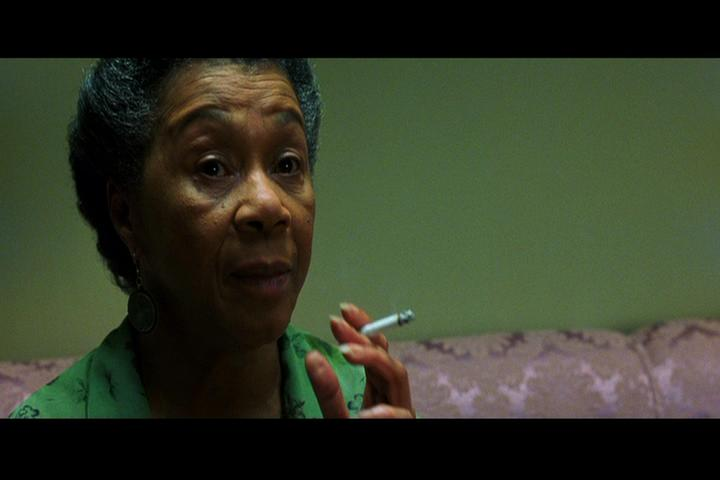
\includegraphics[width=0.5\linewidth]{fig/14a938db9f7b7466d0164e8c.jpg}
\end{figure}

太极代表平衡和阴阳,有Neo就有Smith,充分证明Smith作为Neo对立面是由先知造成的。当然,有人会说这是设计师为了平衡方程式而造成的。但是根据设计师在第二部的说法,Neo属于哥德尔命题中的逻辑外真理,是不能用数学方式解决的。事实上,先知这时“打破平衡”的方式正是“平衡”Neo和Smith(并非无情的数学方式,而是先知的拿手好戏,心理方式,证据是Neo和Smith在能力上的不平衡性),系统把全系统的逻辑外真理归结于Neo(易于管理),一旦Neo被平衡,这个逻辑外真理就演变为“关系”,而非“值”。但是换一个角度看,先知“打破平衡”正是为了真正的平衡,就是最后的和平。“和平”就是一个观众可以期待到的最佳结果,除非这个人还没有摆脱极度人类中心论。

Double Destiny同样代表着和平。鲍德里亚说“利益的平衡就是平衡的利益”,设计师所设想的(也是实现了的)平衡建立在了不平衡的利益之上,以力量来弥补这种平衡上的不足,这是机器中心论。先知要做的就是改变这种渗透了力量的利益平衡,所以先知要考虑机器和人类双方的问题,是Double Destiny。

莲花在印度教里和守护神Vishnu有极大的联系,对他我就不仔细说了,Vaishnava认为Vishnu是至高神,Smarta认为Vishnu只是梵天的一个化身。所以多说反而麻烦,很容易混淆。不过只要知道他是“守护神”就够了,完全可以诠释先知的立场。

Neptuneneo兄跟我说《黑客帝国》也是很不错的爱情片,他指的是Ghost对小崔很东方的暗恋。仔细看看小崔和Neo和爱情也很有味道,该热烈就热烈,该含蓄就含蓄。这里一听Seraph要带他们去救Neo,小崔立马转身跟去了。根本没有考虑先知以前对他们撒的谎,这里还是老莫沉得住气。情爱是疯狂的,友爱是理智,父爱是形而上学的。(叔本华语,马上就要在Rama出场后讲一下这个父爱)

另外讲几点有趣的小细节

先知的香烟盒上有一段文字很有趣“烟草会产生一些序列,这些序列会造成胸口疼和突发心脏病。”很有Matrix味道吧。

剧组为了纪念老先知的去世,特地在场景里加了一个天鹅形的钟。

先知在这里坐的位置是第一部里一个念佛经的小孩坐的地方,老莫和小崔站在了玩勺子的小孩坐的地方。Seraph站的是第一部里给Neo开门的那个领路人的地方。

\myparsep

我们回到火车站,看看这些对话里有什么值得学习。(为什么不说“值得注意”呢?因为光注意是不够的,黑客帝国应该是拿来学习的东西)

\begin{myquote}
Sati: Are you from the Matrix?

Neo: Yes. No. I mean, I was.
\end{myquote}

Neo还在强调时间,说明他还没有掌握时间。但是他对时间也有直觉,他预感到了大楼的爆炸,预感到了电子乌贼。但是他不能控制这种能力,这种看透一切的能力。(黑格尔说“时间是一个人无法看透一切而产生的幻觉”)根据全定论或是因果律,一切皆注定。我很不明白的是,为什么有这么多人认为一切都是偶然呢?不管别人,反正导演相信一切注定,叔本华相信一切注定,对我来说足够欣慰了。

\begin{myquote}
Sati: Why did you leave?

Neo: I had to.
\end{myquote}

这是典型宿命论的论调,或是悲观面对全定论的态度。Neo刚刚才消极地讨论时间,这里消极地讨论命运也是必然的。其实Neo的思想进步正是导演的哲学学习历程,我可以万分肯定这一点,因为我本人就是这样。在看到全定论本质之前看到全定论的现象,消极的悲观论调是不会少的,除非是乐天派。(乐天派喜欢哲学吗?)

\begin{myquote}
Sati: I had to leave my home too.
\end{myquote}

这一句其实是很厉害的,“我也是不得不离开家”,就是说对Neo来说,Matrix才是他的家。或者我们可以再老套一点,谈笛卡尔的身心二元(对黑迷来说都审美疲劳了)。我在这里分的身心二元和笛卡尔的并不一致,是把Neo分为人和程序。(画外音:看起来好像和笛卡尔一点没关系嘛!)这里的程序是身,人是心。Neo是以人的思维,程序的能力在做事。Sati这句话是对Neo的程序身份说的,因为Sati并不明白人类的思维,我们在后面看到先知在教Sati什么是“爱”。

\begin{myquote}
Rama-Kandra: Sati! Come here, darling. Leave the poor man in peace.

Sati: Yes, papa.

Rama-Kandra: I'm sorry, she is still very curious.
\end{myquote}

这个“好奇”是很重要的,这是任何有意识的物体所必备的特质。

\begin{myquote}
Neo: I know you.

Rama-Kandra: Yes, in the restaurant of the Frenchman. I am Rama-Kandra. This is my wife Kamala, my daughter Sati. We are most honored to meet you.
\end{myquote}

Rama是Vishnu一个化身的名字,也可以看出他和先知的关系不一般了。Kamala是一个印度神Lakshmi的一个别名,Vishnu的妻子(其实她和莲花关系更大,Kamala的意思就是“She of the lotus”)。由于导演有糅合基督教野史和古希腊神话的前科,看来他们对印度教是最尊敬的。叔本华、尼采、肯·韦伯无不欣赏印度教(叔本华在印度待了好几年研究印度教呢),因为印度教就是一种哲学,而不是一种控制人的方式。

\begin{myquote}
Neo: You're programs.

Rama-Kandra: Oh, yes. I'm the power plant systems manager for recycling operations. My wife is an interactive software programmer. She is highly creative.
\end{myquote}

看看这些程序是干什么的!多么重要的程序啊!Rama管着Matrix人口的更新换代,Kamala管着人类之间的交流。而且两者都和救世主有着莫大的关系,Neo醒来时遇到的机器就是Rama (起码也是他管理的吧)。Neo的超能力和“交感”是密不可分的,所以说是Kamala赋予了他超能力。这对夫妇分明掌握着Neo的生死!而Neo又是系统不可或缺的部分,可见这两个程序的重要性。先知在《Enter the Matrix》游戏里说过,她的躯体是被她“最信任”的两个程序出卖的。那么他们和先知之间的关系也很明朗了。Rama释放Neo,而Kamala给Neo力量(当然,这也符合设计师原来的原则)。

\begin{myquote}
Kamala: What are you doing here? You do not belong here.

Rama-Kandra: Kamala! Goodness, I apologize. My wife can be very direct.

Neo: It's okay. I don't have an answer. I don't even know where ``here'' is.

Rama-Kandra: This place is nowhere. It is between your world and our world.
\end{myquote}

还是那句话,这里是Limbo,哪里也不是。可以说是世界间的世界,也可以说是地狱的第一层。

\begin{myquote}
Neo: Who's the Trainman?

Rama-Kandra: He works for the Frenchman.

Neo: Why'd I know you were going to say that?

Rama-Kandra: The Frenchman does not forget and he does not forgive.

Neo: You know him?

Rama-Kandra: I know only what I need to know. I know that if you want to take something from our world into your world that does not belong there, you must go to the Frenchman.

Neo: Is that what you're doing here?

Kamala: Rama, please!

Rama-Kandra: I do not want to be cruel, Kamala. He may never see another face for the rest of his life.

Neo: I'm sorry. You don't have to answer that question.

Rama-Kandra: No. I don't mind. The answer is simple. I love my daughter very much. I find her to be the most beautiful thing I've ever seen. But where we are from, that is not enough. Every program that is created must have a purpose; if it does not, it is deleted. I went to the Frenchman to save my daughter. You do not understand.

Neo: I just have never ...

Rama-Kandra: ... heard a program speak of love?

Neo: It's a ... human emotion.

Rama-Kandra: No, it is a word. What matters is the connection the word implies. I see that you are in love. Can you tell me what you would give to hold on to that connection?

Neo: Anything.

Rama-Kandra: Then perhaps the reason you're here is not so different from the reason I'm here.
\end{myquote}

“爱”只是一个词,重要的是其中的关系。这是连叔本华的对头黑格尔都同意的。问题是这个关系本身是否值得?叔本华认为除了同情,没有什么感情是不基于利益之上的。叔本华没有爱,只有性。这一点和设计师一样哦!(设计师的造型来自弗洛伊德)在《黑客帝国》里,并不是没有人持叔本华这种观点,Smith就是这个例子。印度一家的观点更像是尼采,虽然尼采也有很多让女人们很反感的言论,但是尼采是浪漫的。我们用一个“同理可证”就可以把尼采的“爱命运”转变为“爱爱情”。我们可以爱我们无法抗拒的命运,为什么不能接受这骗人的爱情呢?叔本华说:“世界是我的梦”。尼采说:“人生即便是梦,也要过得有滋有味。”这就是Neo和Smith的最大不同。

\myparsep

火车人出场了。

\begin{myquote}
Seraph: That's him.

Trainman: Get away! Get away from me!

Seraph: We don't want trouble.

Trainman: Get the hell away from me!

Seraph: We need your help.

Trainman: I can't help you. No one can help you!
\end{myquote}

追火车人这里可以看到一些有趣的广告牌,一些是赞助商的广告,比如说三星和Powerade的广告。最重要的还是下面图中那个Tastee Wheat。

第一部里Mouse问Neo有没有吃过Tastee Wheat的时候谈到了一个被我们黑迷称之为“麦片理论”的理论。这个理论其实很重要的,算是诺齐克“经验机器”设想的一个延伸。我们把味觉延伸出去,一切感官都在“麦片理论”的范围之下,甚至是自然定律也是。比如说你怎么知道在外面的世界里,你就不能飞呢?其实“麦片理论”可以解释一切这部电影里所谓的“科学问题”(虽然绝大部分不用这个理论也能解释)。

\begin{figure}[htb]
\centering
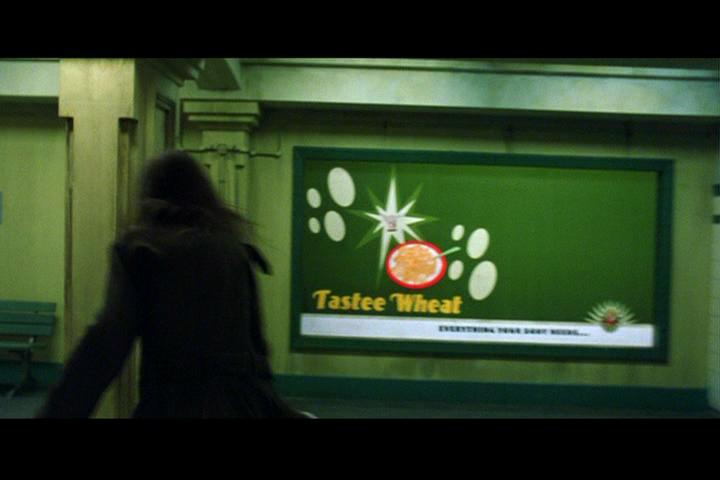
\includegraphics[width=0.5\linewidth]{fig/4000843531b7cf1190ef39a9.jpg}
\end{figure}

这里我要介绍一下一部我比较喜欢的电影《一九八四》(更喜欢小说,三大反乌托邦小说之一嘛),导演也是很喜欢这部作品的,我认为导演安排他们在吃饭的时候提出这个理论就是一种对《一九八四》的致敬。《一九八四》里有一段,主角温斯顿在吃饭的时候,对面一位仁兄说他们吃的那个东西看起来像是肉,尝起来像是肉,但却是豆腐做的(看得到“麦片理论”的影子吧)。neverwin也提到一点,Neo房间的号码101也是对《一九八四》的致敬(其中101房里的是一个人最大的恐惧)。导演兄弟编剧的新作《V字仇杀队》也有很多对《一九八四》的致敬,比如娜塔丽剃光头的镜头。有趣的是,在《一九八四》里反抗极权政府的温斯顿扮演者John Hurt,却在《V字仇杀队》中扮演了极权政府的头目。

这个很容易让人联想到那种兜售偷来的手表的人。不过不要以为这就是导演的意思。火车人一共有九块手表,而且时间各不相同,代表但丁所说的九层地狱。因为每一层地狱的时间都是不同的。

\begin{figure}[htb]
\centering
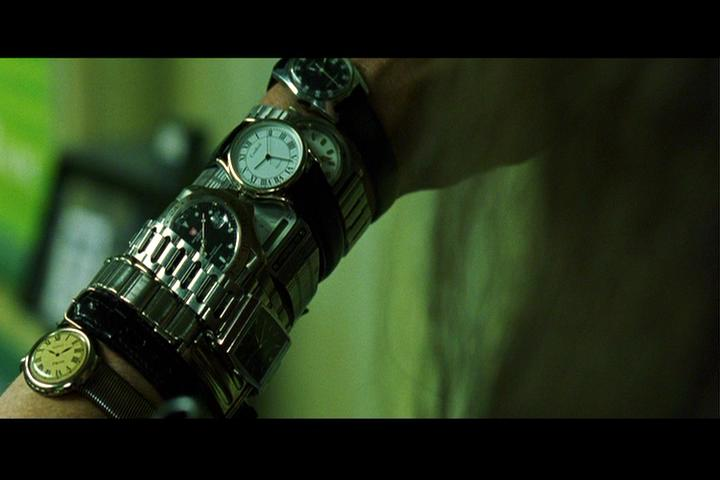
\includegraphics[width=0.5\linewidth]{fig/058d77c67f85e61b9d163da9.jpg}
\end{figure}

有人可能认为这是我在胡说,但是我可以证明哦。

下图是Rama在等火车时看手表,6点10分,正是上图火车人第一块手表显示的时间。两个镜头不是同时拍摄的,不要说这是巧合。再加上Limbo确实是地狱的第一层,应该没有什么异议和需要解释的地方了吧。而且这个6点10分也是有含义的。

圣经的撒母耳记下6:10:于是大卫不肯将耶和华的约柜运进大卫的城,却运到迦特人俄别以东的家中。

Rama不肯将Sati留在Rama的世界,却带到先知的家中。而且Sati本身也是一个契约,用先知的躯体换来的自由哦。

\begin{figure}[htb]
\centering
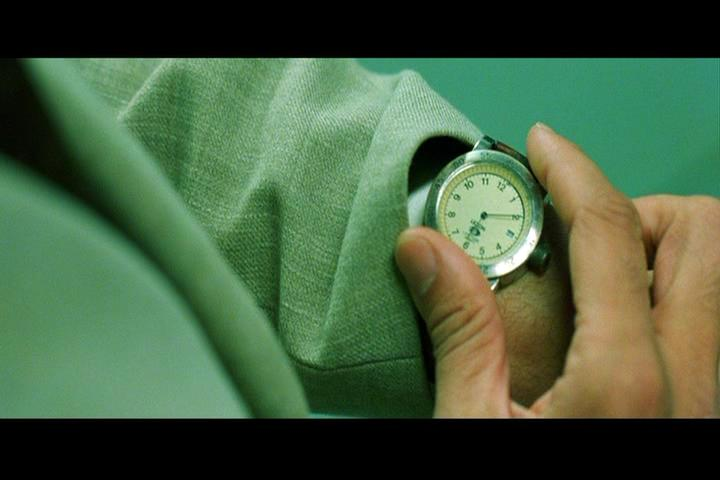
\includegraphics[width=0.5\linewidth]{fig/759c98255a5b746034a80fa9.jpg}
\end{figure}

\begin{myquote}
Neo: When is the train due?

Rama-Kandra: It's already late. It's not like the Trainman to be late.

Neo: You think it has something to do with me?

Rama-Kandra: I cannot say. Who knows such things? Only the Oracle.

Neo: You know the Oracle?

Rama-Kandra: Everyone knows the Oracle. I consulted with her before I met with the Frenchman. She promised she would look after Sati after we said goodbye.

Neo: Goodbye? You're not staying with her?

Rama-Kandra: It is not possible. Our arrangement with the Frenchman was for our daughter only. My wife and I must return to our world.

Neo: Why?

Rama-Kandra: That is our karma.

Neo: You believe in karma?

Rama-Kandra: Karma's a word, like ``love,'' a way of saying ``what I am here to do.'' I do not resent my karma --- I'm grateful for it. Grateful for my wonderful wife, for my beautiful daughter. They are gifts. And so I do what I must do to honour them.
\end{myquote}

印度教和佛教相信人有两种状态,涅槃和轮回。涅槃世界是Neo最终的境界,这里就不说了。轮回世界相比涅槃世界有三个限制:时间、空间、因果(karma)。导演经常在这三个方面作文章的。Karma的原意是因果报应,而在人们眼里却成了命运的代名词,我们这样的全定论者是可以接受的,不知叫嚣着万事偶然的人如何看待karma。在电影里,这个词还有“目的”的意思。

而这里Rama表现出的对命运的态度就是尼采所说的amor fati,就是“爱命运”的意思。在ETM游戏中,Ghost曾经直接引用尼采关于“爱命运”的诗句:

One must want nothing to be different. Not forward, not backward. Not in all eternity. Not only to bear what is necessary, but to love it.

(人必要无所异。不在未来,不在过去,不在永世。不光要承受那必然,还要爱它。)

先知则亲口道出了amor fati这个名字,这是除了鲍德里亚的《模仿与拟像》之外,唯一明确引用的例子。

我们再由“目的”这层意思上来看,《黑客帝国》是至今为止对人物对生命态度刻画最为深刻,最为本质的电影,因为黑客帝国是放在形而上学的本质上谈论的。但是由于极化了这些表现,这最本质的东西看上去反而不真实了(就像我举的驴子和食物的例子,在现实中是不可思议的,只有在很清晰的解释之后才会被人勉强接受),而且除了Rama之外大部分人对生命,命运之类的概念持着令人不愉快的观点,也很难让普通人接受。只有叔本华一派悲观的哲学家才会维护这些观点。

现在就看看各种程序对“目的”的态度:

法国人和一干流亡程序不甘命运。窝在自己的小天地里。

Smith憎恨命运,尽全力改写一切,而最终仍然被命运所终结。

开锁匠对命运持无所谓的态度,要死了还说那是应该的。

Rama感激命运,是唯一一种大多数人可以接受的态度。

Neo由最初的不相信命运,到执行自己的karma, 到最后摆脱命运进入涅槃世界。

先知和设计师塑造别人的命运,这是我们暂时不考虑的。

特工没有情感,对“命运”根本没有态度可言。

对各种态度的刻画简洁而深刻,可惜却很少有人注意。所以说《黑客帝国》最大的毛病就是太完美,正如哲学大师齐泽克所说:“《黑客帝国》就是那幅众所周知的上帝像,无论你站在哪里,上帝都在看着你。”这样一来,也就没有人去找上帝看着的地方了。就拿我来说,注意的只有哲学,而且主要看叔本华,法国哲学界为《黑客帝国》开了两次圆桌会议,议题几十个,哪个不比我这篇文章讨论的深刻。所以我这篇在绝大多数人眼里已经过于刁钻的文章,其实只是《黑客帝国》的九牛一毛。

\begin{myquote}
Sati: Papa, the train!

Rama-Kandra: Yes! Find your bag, quickly!

Neo: Can I carry that for you?

Rama-Kandra: All right.

Trainman: Hurry it up, I'm late!

*Kamala and Sati pass, Trainman stops Neo*

Trainman: Who are you?

Rama-Kandra: He's a friend.

Kamala: Rama!

Trainman: I know you. So that's what they wanted.

Neo: I need to get back. I'll pay you anything you want.

Trainman: Oh?

Neo: One way or another I'm getting on this train.

Trainman: Oh, no, no, no. You're gonna stay right here until the Merovingian says different. If I know him, you're gonna be here for a long, long time.

Neo: I don't want to hurt you.

Trainman: You don't get it. I built this place. Down here I make the rules. Down here I make the threats. Down here, I'm God. *to Rama-Kandra* Get on the train, or you'll stay here with him.
\end{myquote}

又要提一下齐泽克了,他曾经写了篇关于黑客帝国的文章,有人是这么评价的:“那原本是批评《黑客帝国》的文章,却被黑迷看作解读《黑客帝国》的指导。”实际上,那篇文章更接近于我之前所说的“哲学家垄断”现象。仔细看那篇文章就会发现他在文章中留下了很多矛盾和错漏,所有批评《黑客帝国》的地方都是可以反驳的(他主要还是说《黑客帝国》还可以更好,而不是贬低,比如他在谈到Spoon Boy的时候就说《黑客帝国》可以放开讨论“什么是自己”),我就曾经写过一篇文章反驳了他在那篇文章里提出来的很多论点。按我的经验看,我相信他那篇文章是在考验黑迷的哲学素质。

上面的话是我在想到齐泽克的时候觉得不吐不快的话,这里要说的其实是齐泽克在那篇文章里提到的一个论点:大他者。其实这个大他者的问题被认为是齐泽克误会了拉康的意思。我在这里偏向齐泽克一点的说,大他者可以被认为是整个社会。塑造一切,统治一切的整体。在电影中,Mobil Ave是火车人建造的,规则是他制定的,他就是神,就是大他者。齐泽克曾经用电梯的关门钮来比喻神,这样看来,神就是大他者,而非我们通常所理解的白胡子老头。我相信叔本华,尼采两位反感基督教的哲学家是会很同意这种看法的。

大他者是唯一可以在轮回世界不受时空和因果影响的,因为他本身就是时空和因果。简单的解释一下,全世界的人都是我,自然定律也由我制定,那我就是一个单独的存在,怎么还会受世界性质的影响呢?

\myparsep

\begin{myquote}
Seraph: We should return to the Oracle. She'll know what to do.

Trinity: No. We know what has to be done.
\end{myquote}

这里再一次证明了先知的能力是“直觉”。她可以预测的就是人们对某件事物的反应,Trinity他们去追人就不可预测了。令我很高兴的是,neverwin在他《第二部非官方解释》最新的更新中也指出这一点。哈哈,英雄所见略同!

下面这张图也很有意思,low clearance的含义我们很清楚了。低调,干净,这就是黑客们的风格。黑白相间的意思我们也很清楚,说明要打架了。这在第一部的非官方解释中就提到了。

\begin{figure}[htb]
\centering
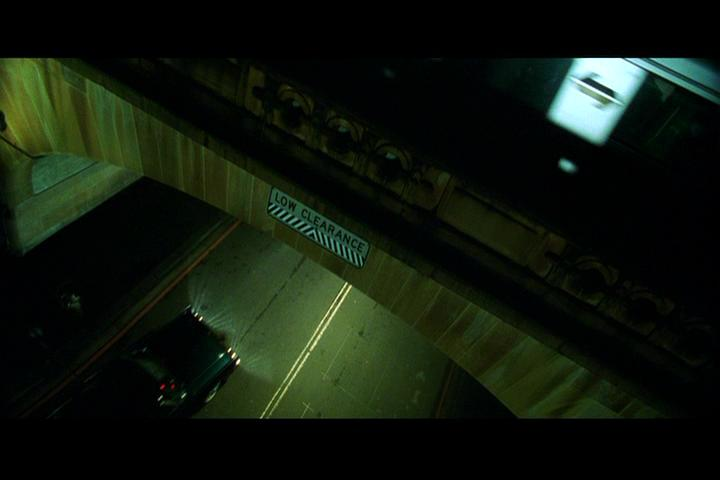
\includegraphics[width=0.5\linewidth]{fig/8b758b82f42f6090f603a6f5.jpg}
\end{figure}

接下来有一段Neo在Mobil Ave的镜头,就是Neo沿着铁轨跑,结果从另一面回来了。有人说那是搞笑,事实上,那也是很重要的,正是我说的轮回世界三个限制之一,空间。我说过导演经常在这几个方面作文章,关于“空间”的具体例子就是开锁匠的走廊,法国人的城堡,设计师的房间,火车人的车站。事实上,这里的奔跑正代表轮回(samsara)。其实“轮回”这个翻译并不佳,samsara还有“看不清真我,得不到梵,相信虚幻的世界”这些含义。不是“生,死,再生”可以涵盖的。

接下来,那个三人小组到了法国人的场子。

\begin{myquote}
Q-Ball Gang Member \#1: You've got to be kidding ...

Q-Ball Gang Member \#2: Holy shit, it's Wingless.

Q-Ball Gang Member \#1: I get it. You must be ready to die.

Seraph: I need to speak with him.

Q-Ball Gang Member \#1: The only way you're getting through this door is over my big dead ass.

Seraph: So be it.
\end{myquote}

够酷吧,Seraph一句“那好吧”真是够力度。其实,我们在这里也可以看出来Seraph和法国人是老相识了。

下面这张图也有些内容可以聊聊。首先这个拱形的入口代表性,第二部里Neo和Trinity在ML的时候,也是这个拱形结构。《达芬奇密码》里也指出过拱形和性的关系。左边的石座上有倒十字的标志,是反基督的一个标志。不要忘了,这里的主人Merovingian的名字来自法国六个封建王朝第一个,被认为是耶稣的后裔。这可不是《达芬奇密码》的原创,事实上,Merovingian家族被如此看待已经几个世纪了。而法国人这个地方就是个反基督的地方。叔本华说过:“然而一个像上帝如耶和华的神,由于纯粹的幻想而创造了这个苦难的世界,且乐此不疲,额手称庆,褒赞其成功,然后宣布凡物都是美好的——这真是行不通的事。”而尼采更是写了《反基督》这样的书。可笑的是基督徒还很支持《黑客帝国》里的圣经隐喻,却对《达芬奇密码》穷追猛打,由此我们也可以看到普通影迷看电影的本事到底如何了。

\begin{figure}[htb]
\centering
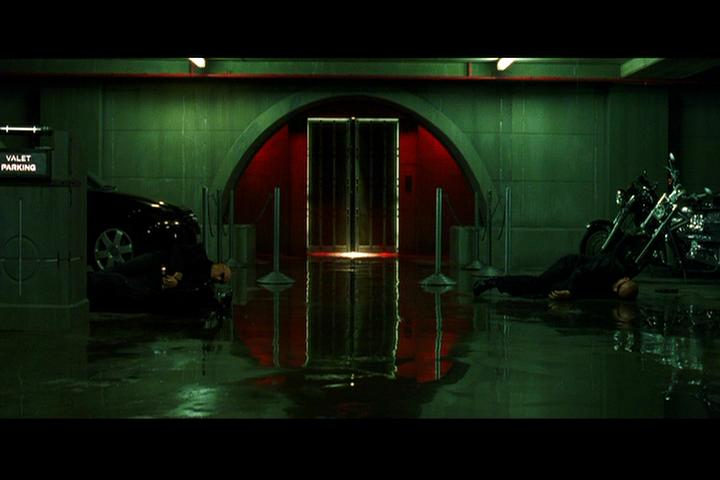
\includegraphics[width=0.5\linewidth]{fig/4fd64bed745da1d4b31cb1f5.jpg}
\end{figure}

接下来就是一段很有型的枪战,没有什么特别要讲的。提一下这里5个反派的名字,第一个被杀死的家伙叫Dogboy,两个长的挺像的光头,一个叫Rook,一个叫Pinball Wizard,被小崔踢进墙的家伙叫Jerry, 戴防毒面具的家伙姓名不详,演员的真名叫Alex Kuzelicki。

这些名字也是有意思的,Rook是小说《时间机器》里的一个科学家的名字,后来Warren Publishing公司出版的很多漫画中都出现他。Pinball Wizard原意是弹球游戏的终极关,导演指的是The Who乐队的一首60年代摇滚歌曲。而Dogboy就不好说了,是很常见的外号。而Jerry这个名字就是最重要的,《猫和老鼠》都知道吧,齐泽克曾经在解释大他者的时候用《猫和老鼠》举过例子,无论猫或是老鼠在哪一集被整的很惨,甚至升天了,都不影响在下一集里完好的出现。很奇怪的是,Tom猫才是老被整的对象,而齐泽克的具体例子里却偏偏说Jerry被整的一次(嘴里炸药爆炸,然后被切成片)。

下面这张图就是Jerry被Trinity袭击的画面。小崔这招牌踢又出现了。

\begin{figure}[htb]
\centering
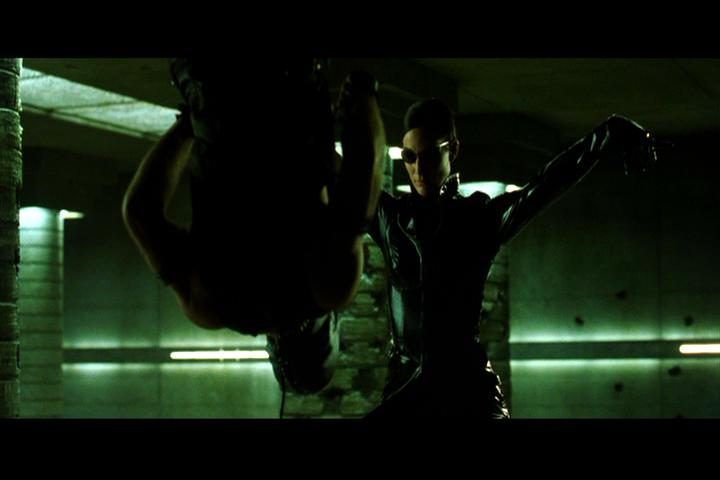
\includegraphics[width=0.5\linewidth]{fig/328dcf1b4553d7faaf5133cc.jpg}
\end{figure}

\begin{myquote}
Merovingian: What in the hell? *laughs* I don't believe this.

Merovingian: *to the DJ* Hey. Hey! *to Seraph* The prodigal child returns. L'ange sans ailes (Trans: The angel without wings). Are you here for the bounty, Seraph? *laughs heartily* Tell me, how many bullets are there in those guns? I don't know, but I don't think you have enough.
\end{myquote}

法国人这句“What in the hell”挺逗的,这里就是Hel嘛。这里可以看出来,Seraph以前是跟法国人的,后来先知成了系统最重要的部分,Seraph就保护先知了。另外,我们还可以看到Trinity爱情的盲目,Seraph本来建议回去问先知,小崔救夫心切,子弹都没带够就去法国人那里砸场子。

\begin{myquote}
Seraph: We only want to talk.

Merovingian: Oh, yes, I'm sure you do, you have fought through hell to do so, yes? I'll tell you what I'll do. Put down the guns and I will promise you safe passage out of here.

Seraph: All three of us.

Merovingian: Oh, yes, yes. Of course.
\end{myquote}

又是这句很阴险的“当然”,说明法国人要放他们出去是有目的的。别以为小崔手枪一顶,法国人就妥协了。我在本文开始就说过,法国人也是革命者,他代表的是废弃程序的利益。如果Matrix一再的循环,他永无出头之日。这时候他虽然控制了Neo,照理说循环已经被打破了,法国人可以肆无忌惮的增长势力,而不怕每次Matrix升级的时候,救世主都来砸场子。但事实并非如此,Neo还有个复数Smith呢,小史可比Neo难对付,法国人要是被Smith侵入了,唯一可以和他抗衡的Neo又被困在别的世界,那不就完蛋了嘛。他不直接放人,而和对现今形势一无所知的小崔他们讲条件,太奸商了。

\begin{myquote}
*Trinity, Seraph, and Morpheus put down the guns and are escorted up the stairs*
\end{myquote}

这里导演又拿基督教开涮了,二楼包厢的一个角落里,一个白衣MM手里端着一个巨大的苹果,分明是暗示夏娃用苹果引诱了亚当,结果下地狱了。图我就不截了,有心的朋友可以自己去看看。

\begin{myquote}
Merovingian: *laughs* Quelle bonne surprise, n'est pas? (Trans: What a fine surprise, isn't it?) Who could've guessed we'd all be seeing each other so soon after our last meeting? A fate too kind. And since you, my little Judas, have brought them here, I can only surmise that the fortune teller has found herself another shell? Disappointing, but not unexpected. I do hope, however, she has the good manners to learn her lesson, and to remember that there is no action without consequence. And if you take something from me you will pay the price.
\end{myquote}

这里就开始讲他的工作原理了:consequence。这个词在逻辑学里也是因果的意思,也可以说是一系列的推论。另外提到“价值”,这是选择的重要指标(说唯一指标太绝对了),也是推论的一个重要方向。价值产生于欲望,“欲望来自我们对未来的思考”(叔本华语),法国人就是以当前的情况来推论过去的价值。但“时间这一主动力使每一刻变得毫无价值”(叔本华语),所以法国人就没用了。(这一点是形而上学的,并不是说法国人在实际中没有用,导演这么安排是为了突显这种哲学理论)

\begin{myquote}
Seraph: You know why we are here.

Merovingian: *laughs* Come, now. What kind of question is this? Of course I know. It's my business to know. Some might think this a strange coincidence, but I do not. I am curious, though, as to how it actually happened. Do you know?
\end{myquote}

这里就可以看到各种人和程序对自己的目的和命运的态度。

Morpheus:fate

先知:purpose

Smith:not free

开锁匠:meant

Rama:karma

法国人:business

法国人是利用他的目的在为自己获得利益,是最实在的一种方法,比起Rama的“感激命运”实惠多了。另外注意法国人问的这个问题,“你认为这是怎么发生?”他问的是现在的处境是如何造成的,答案就是Neo他们砸他场子,带走开锁匠,杀死他大量手下。法国人囚禁Neo是在报仇。

\begin{myquote}
Trinity: No.

Merovingian: No? I didn't think so. But it is always best to ask.

Morpheus: We want to make a deal.

Merovingian: *laughs* Always straight to business, huh, Morpheus? Okay. I have something you want. To make a deal, you must have something I want, yes? And it so happens there is something I want. Something I've wanted ever since I first came here. It is said they cannot be taken, they can only be given.
\end{myquote}

这就是我说的奸商部分,自己分明就要放人的,还要敲诈一笔。

\begin{myquote}
Morpheus: What?

Merovingian: The eyes of the Oracle. *laughs*

Merovingian: I have told you before, there's no escaping the nature of the universe. It is that nature that has again brought you to me. Where some see coincidence, I see consequence. Where others see chance, I see cost. Bring me the eyes of the Oracle, and I will give you back your saviour. That seems a particularly fair and reasonable deal to me. Yes, no?
\end{myquote}

我曾经开过一个玩笑,说Eye(i)是-1的平方根,Smith是Neo的复数,也就是-1。先知的眼睛把Smith给开了方,Smith就成无理数了。言归正转,先知的眼睛象征先知的能力,最终也确实是先知的能力害Smith被毁。

“先知的眼睛”这个意象出自普希金的一首诗《先知》(六翼天使Seraph也在其中出现):

{\centering \it

忍受着精神上的煎熬,

我缓缓的走在阴暗的荒原,

这时在一个十字路口,

六翼天使出现在我的面前。

他用轻得象梦似的手指

在我的眼珠上点了一点,

于是象受了惊的苍鹰,

我张开了先知的眼睛。

他又轻摸了一下我的耳朵,

它立刻充满了声响和轰鸣:

我听到了天宇的颤抖,

天使们翩然在高空飞翔,

海底的蛟龙在水下潜行;

幽谷中的藤蔓在簌簌的生长。

他附身贴近我的嘴巴,

一下拔掉我罪恶的舌头,

叫我再也不能空谈和欺诈,

然后他用血淋淋的右手,

伸进我屏息不动的口腔,

给我安上智慧之蛇的信子。

他又用利剑剖开我的胸膛,

挖出了我那颤抖的心脏,

然后把一块熊熊燃烧的赤炭

填入我已经打开的胸腔。

我象一具死尸躺在荒原,

上帝的声音向着我召唤:

“起来吧,先知,你听,你看;

按照我的意志行事吧,

把海洋和大地统统走遍,

用我的语言把人心点燃。”

}

另外,这里法国人的一句“别人看到巧合,我看到因果;别人看到机会,我看到代价”也是经典,这就是几率论者和全定论者的区别。这里我要举一个对于“完事无因”的著名反驳:“完事无因”这句话要么有原因,要么没有。如果这句话没有原因,那就没法证实它是对的;如果这句话有原因,本身就证明了原因的存在。

\begin{myquote}
Trinity: I don't have time for this shit.

*Hel Club upstairs fight*

Trinity: You want to make a deal, how about this? You give me Neo, or we all die right here, right now.

Merovingian: Interesting deal. You are really ready to die for this man?

Trinity: *cocks gun* Believe it.

Perseph: She'll do it. If she has to, she'll kill every one of us. She's in love.

Merovingian: It is remarkable how similar the pattern of love is to the pattern of insanity.

Trinity: Time's up. What's it gonna be, Merv?
\end{myquote}

“爱”和“疯狂”多么相似啊!难怪很多哲学家都标榜只有性,没有爱。叔本华、尼采都是如此,弗洛伊德就不说了,分明是个“淫秽的哲学家”,当今的肯韦伯几乎做了和尚,齐泽克经常讲黄色笑话,就是对“爱情”绝口不提。

这一部分开始前,先告诉大家一个好消息,neverwin已经结束了第二部的非官方解释,相信这两天就会开始写neverwin版的第三部非官方解释了!(neverwin达人看到的话,别忘了给小弟“杂物”的版本也做做广告哦,哈哈)

\begin{myquote}
Neo: Ok. You got yourself into this. You can get yourself out.
\end{myquote}

这里Neo预见到了他最后要走的路。这是一个突破,因为这一次是Neo尽力去感知的,而不是像以前那样灵光一闪。按黑格尔的说法,Neo正在努力看透一切。而这个地方正是轮回的表现,看透轮回就可逃出这个地方,结果下一个镜头火车就到了。我们当然知道这是Trinity拼命做到的,但我们也要理解导演要求如此拍摄和剪接的意思。

这火车也很有意思,火车人在被Seraph他们追得跳火车的时候,我们可以看到这些火车前都有Loop(环形线)的字样,而这辆车进站的时候,我们可以看到那个位置被挖空了,说明循环被打破。但Matrix一样是轮回世界,连Zion都是一样。但虚拟派不要抓着我这句话说Zion也是虚拟的。无论你信不信先知,她一样可以利用你,无论世界是否虚拟,你永远受着控制。(相对叔本华的终极自由而言)

\begin{figure}[htb]
\centering
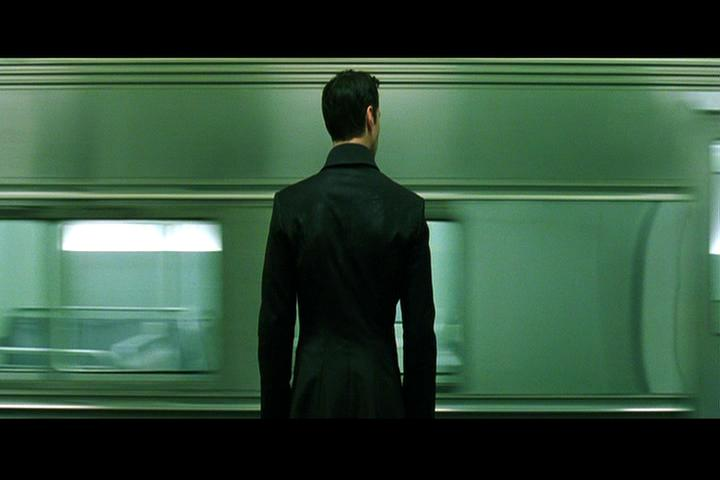
\includegraphics[width=0.5\linewidth]{fig/926a29387d14c524b8998fe3.jpg}
\end{figure}

\myparsep

\begin{myquote}
Morpheus: Are you ready for us?

Link: Almost, sir. They got some pretty ancient hacks here, we're working on it. Did you find Neo?

Morpheus: Can't you see him?

Link: No, sir. We were reading something but I couldn't tell what it was.

Neo: I can't leave yet.

*Trinity looks over at him*

Neo: I have to see her.

Trinity: Now?

Neo: This is my last chance.
\end{myquote}

这里可以解决一个关于Bane被入侵时未被发现的问题。neverwin的解释是Bane醒来说自己逃出来了,船员也会相信的。其实在这里可以看出来,船员们根本没有看到Bane被Smith入侵。黑迷们还记得Logos启动之后Sparks的反应吧,他说Matrix的信号有问题。当时Matrix不稳定的原因只有一个,那就是Smith的蔓延。所以说Bane被入侵的时候,船员们根本无法从屏幕中读出什么来。况且看数码雨是要经验的,头一回看到这样的事情,即便屏幕清清楚楚,他们也未必知道到底发生了什么。

这段和第一部里几乎一模一样,唯一不同的是开车的人变了,第一部是Cypher开的车,这里是Seraph,而这两个家伙都是“叛徒”。区别是Cypher“变坏”,Seraph“变好”。

\begin{figure}[htb]
\centering
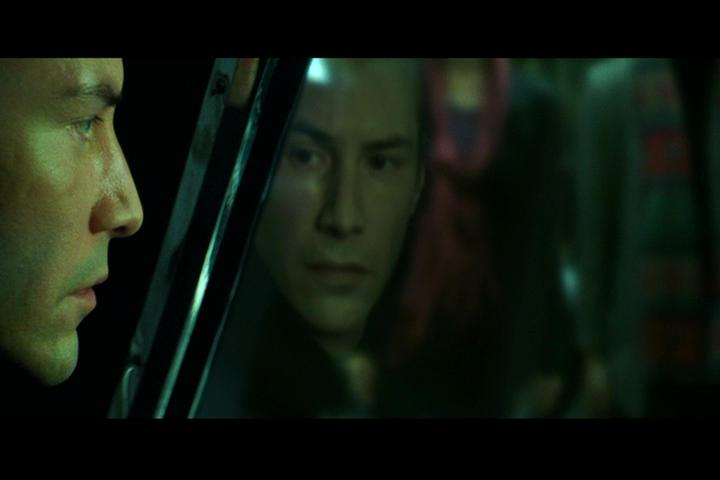
\includegraphics[width=0.5\linewidth]{fig/f64563d08227bd8fa0ec9ce3.jpg}
\end{figure}

到先知那里了。

\begin{myquote}
Oracle: That's it. That's the secret. You've got to use your hands.

Sati: Why?

Oracle: Cookies need love like everything does.
\end{myquote}

饼干也需要爱!先知开始教Sati那些人类的情感。先知教的这种爱是博爱,这一点叔本华是很缺乏的。但奇怪的是佛教很讲究博爱,而叔本华又研究多年佛学,他怎么就那么悲观呢?看来,Neo和Smith正是叔本华的两面,也是导演的两面,也是我的两面。任何一个既欣赏叔本华,又敬重佛教的人都会有这样的情况。

\begin{myquote}
Sati: Neo!

Oracle: I was hoping to have these done before you got here. Oh, well. Sati, honey, I think it's time for a tasting. Take the bowl to Seraph and find out if they're ready.
\end{myquote}

又一次证明先知的能力是“直觉”,Neo什么时候来这样物理因素很重的事件是很难预测的,但是先知确实预测到了Neo会来。

\begin{myquote}
Sati: Okay. *to Neo* I'm glad you got out.

Neo: Me too.

Oracle: So, do you recognize me?

Neo: A part of you.

Oracle: Yeah, that's how it works. Some bits you lose, some bits you keep. I don't yet recognize my face in the mirror, but ... I still love candy. *offers Neo a piece of red candy*
\end{myquote}

很精辟,佛经上讲:“得就是失,失就是得,有得必有失,有失必有得。”同一件事情的得与失比例对于不同的人来说是不一样的,你若能平心看到“得等于失”,那你就得道了。

\begin{myquote}
Neo: No, thank you.

Oracle: Remember what you were like when you first walked through my door, jittery as a junebug? And now just look at you. You sure did surprise me, Neo, and you still do.
\end{myquote}

哈哈,Smith说伟大的先知绝无意外,而先知自己却说Neo给了她很多惊喜,说明先知对Neo的直觉并不永远准确。还好,这一点并不会对大问题产生影响。

\begin{myquote}
Neo: You gave me a few surprises, too.

Oracle: I hope I helped.

Neo: You helped me to get here, but my question is why? Where does this go? Where does it end?
\end{myquote}

救世主问原因了,这是Neo在法国人那里学来的(第二部里,法国人就给他灌输这种思想),原因是动力啊。叔本华认为一个人的行为有两个因素:动机和性格。原因就是动机,这是没有争议的,而性格,既然是塑造出来的,同样也可以被改变。导演为什么在力求和第一部对应的时候安排先知提Neo的改变呢?就是要告诉观众,先知不旦给了Neo动机,甚至改变了Neo的性格。但不知有多少人理解导演的苦心。

\begin{myquote}
Oracle: I don't know.

Neo: You don't know or you won't tell me?

Oracle: I told you before. No one can see beyond a choice they don't understand, and I mean no one.
\end{myquote}

“没有人可以理解自己看不透的选择”,这没有什么需要解释的。需要解释的是“先知还有不理解的选择?”回忆先知之前和Morpheus、Trinity的谈话,先知明确知道她这个选择的代价,但最后这个选择的代价却比她预期的高,说明这是个错误的选择(仅仅就利益而言),那么就无法看透这个选择了。但这个利益上的错误选择却并不完全错误,利益的根本就是生存的欲望,而叔本华在《论自杀》中就说过,像是主义、信仰,就可以超越生死,何况仅仅是被Smith入侵呢。

\begin{myquote}
Neo: What choice?

Oracle: It doesn't matter. It's my choice. I have mine to make, same as you have yours.

Neo: Does that include what things to tell me and what not to tell me?

Oracle: Of course not.

Neo: Then why didn't you tell me about the Architect? Why didn't you tell me about Zion, the Ones before me --- why didn't you tell me the truth?

Oracle: Because it wasn't time for you to know.

Neo: Who decided it wasn't time?

Oracle: You know who. *She points at the Temet Nosce sign above the door*

Neo: I did. *Oracle nods* Then I think it's time for me to know a few more things.

Oracle: So do I.

Neo: Tell me how I separated my mind from my body without jacking in. Tell me how I stopped four sentinels by thinking it. Tell me just what the hell is happening to me.

Oracle: The power of the One extends beyond this world. It reaches from here all the way back to where it came from.

Neo: Where?

Oracle: The Source. That's what you felt when you touched those Sentinels. But you weren't ready for it. You should be dead, but apparently you weren't ready for that, either.
\end{myquote}

救世主的力量当然不能局限于Matrix,在任何一个世界都不应该被终结。而Neo那些问题可以很容易从无线接入来解释。关于Source的问题,先知说Neo在碰到电子乌贼的时候,就感知到了Source。事实上,那些电子乌贼就是Source,那就是本质。我们的思想不应该被局限于“Source是一个空间”,Source完全可以是一种精神,一种本质,一种灵魂。电子乌贼作为一种很基本的机器,就是很本质的。先知说Neo还没有准备好接受,那是当然的了,谁能接受自己的敌人居然如此高尚,如此纯洁?(这么说可能很多人摸不找头脑,看Neo眼瞎之后的视野就知道我在说什么了)

死不死的问题也很有趣:“你应该死了,但是还有准备好。”够绝!敢情不准备好死还死不了。Neo是否该死的问题没有必要解释,也无法解释,因为每个人(包括不用脑子看电影的)都明白,Neo不能死。

\begin{myquote}
Neo: The Architect told me that if I didn't return to the Source, Zion would be destroyed by midnight tonight.

Oracle: *rolls eyes* Please ... You and I may not be able to see beyond our own choices, but that man can't see past any choices.

Neo: Why not?

Oracle: He doesn't understand them --- he can't. To him they are variables in an equation. One at a time each variable must be solved and countered. That's his purpose: to balance an equation.

Neo: What's your purpose?

Oracle: To unbalance it.

Neo: Why? What do you want?

Oracle: I want the same thing you want, Neo. And I am willing to go as far as you are to get it.

Neo: The end of the war. *Oracle nods* Is it going to end?
\end{myquote}

看到了吧,先知要的也是和平。很多人以小人之心度君子之腹,说先知不过是为了一次完备的升级。人家先知是很……的!(没词了)这也符合在她公寓墙上找到的“peace”涂鸦。

\begin{myquote}
Oracle: One way, or another.

Neo: Can Zion be saved?

Oracle: I'm sorry, I don't have the answer to that question, but if there's an answer, there's only one place you're going to find it.

Neo: Where?

Oracle: You know where. And if you can't find the answer, then I'm afraid there may be no tomorrow for any of us.

Neo: What does that mean?

Oracle: Everything that has a beginning has an end. I see the end coming. I see the darkness spreading. I see death. And you are all that stands in his way.

Neo: Smith.

Oracle: *nods* Very soon he's going to have the power to destroy this world, but I believe he won't stop there; he can't. He won't stop until there's nothing left at all.

Neo: What is he?

Oracle: He is you. Your opposite, your negative, the result of the equation trying to balance itself out.
\end{myquote}

我们说过,Neo是逻辑外真理,是在等式之外的,Smith却是因为等式为了平衡而被建造出来的。解释就是先知硬是把逻辑外真理由值转为关系,借设计师的手创造了Smith这个可怕的负数。(我为什么在这里用“可怕”形容Smith呢?我和他有一样的哲学啊!)

\begin{myquote}
Neo: What if I can't stop him?

Oracle: One way or another, Neo, this war is going to end. Tonight, the future of both worlds will be in your hands ... or in his.
\end{myquote}

\myparsep

刚提到Smith,他就醒了。接下来的镜头Neo也醒了。可以看出两个人之间的联系。确实,我每次想到Smith那种理论,就要Neo似的问一句:“没有意义就不能坚持吗?”两者是共存的。

\begin{figure}[htb]
\centering
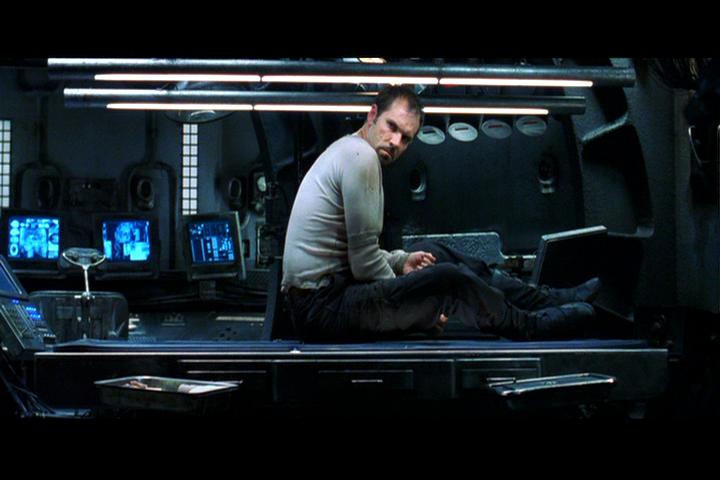
\includegraphics[width=0.5\linewidth]{fig/04eda1ec7ef97f3d26979102.jpg}
\end{figure}

\begin{myquote}
Trinity: How are you feeling? Are you all right?

Neo: I need time.

Roland: That figures.

Maggie: Captain Roland!

Roland: What's up, Maggie?

Maggie: Bane, sir. he's conscious.

Roland: Good. Maybe he's got some answers.
\end{myquote}

有意思,Roland还真有点直觉。Neo出来说“需要时间”,Roland就说“That figures”,人家这个船长不是白当的。先知理解人类的心理,Roland也不差。

现在回到先知那里,我们亲爱的Smith终于要出场了。

\begin{myquote}
Oracle: Mmm, I love that smell. I sure am gonna miss it.

Seraph: Oracle.

Oracle: I know, I know. Sati, honey! Take a few cookies and go with Seraph.

Sati: Can I come back? I would like to come back!

Oracle: I would like that too.

Sati: So I'll see you tomorrow.

Oracle: I hope so, honey, I hope so.
\end{myquote}

先知知道吃不上这饼干了,她烤这些饼干就是为了让Smith打翻的。有人会觉得这不是太无聊了吗?但是对先知来说,基本上一切都是已知的,她本来就是很无聊的程序。还有她们这里说的“明天”既是字面上的意思,又代表“未来”。先知的“hope”也是区分信仰者和非信仰者的重要标志。哈曼议员在最紧急的关头说他们还可以“希望”,而Lock指挥官就明确地说:“希望是不合时宜的奢侈。”

下面一张图也很有意思,先知给了Sati一些饼干,但却不是刚刚烤好的那些。呵呵,饼干都是有目的的。给Sati的饼干就是让她吃的,刚烤好的就是给Smith打翻的。

\begin{figure}[htb]
\centering
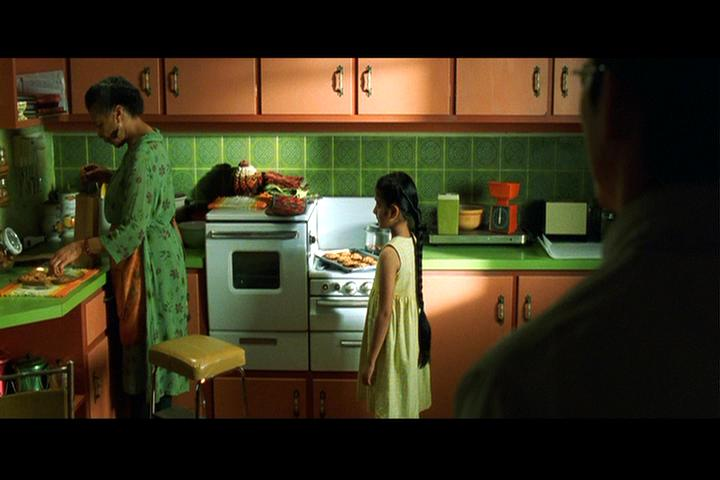
\includegraphics[width=0.5\linewidth]{fig/42486159b22efa2a2834f002.jpg}
\end{figure}

Seraph带Sati走电梯,电梯却坏了。这个neverwin解释的很清楚,《黑客帝国》里的电梯只能上,不能下。他们回头看走廊,灯一盏接一盏灭了,而墙上又出现那个的标志。先知说的darkness spreading就是指Smith,那个标志当然也是指Smith,难怪Hugo Weaving是V字仇杀队主演的最佳人选。

\begin{figure}[htb]
\centering
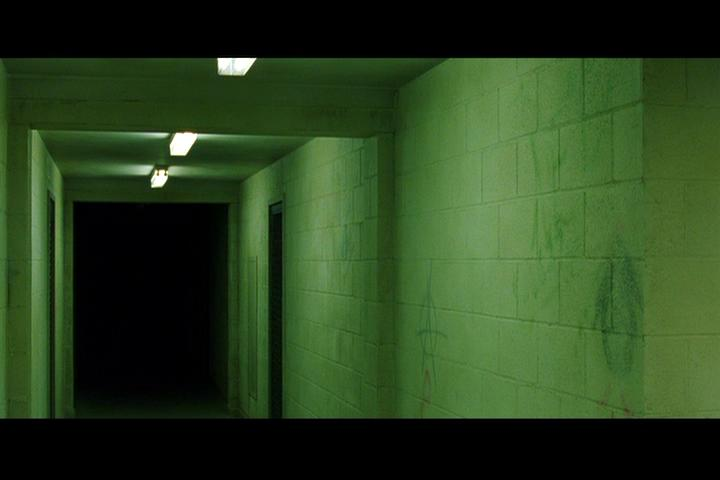
\includegraphics[width=0.5\linewidth]{fig/c621faf21812bd13b07ec502.jpg}
\end{figure}

\begin{myquote}
Sati: I'm scared, Seraph.

Seraph: Come.

Sati: He's following us.

Smith: Well, well, it's been a long time. I remember chasing you was like chasing a ghost.

Seraph: I have beaten you before.

Smith: That's true, but as you can see, things are a little different now. *to Sati* And you must be the last exile.

Sati: The Oracle told me about you.

Smith: Really? And what did she say about me?

Sati: That you're a bad man.

Smith: Oh, I'm not so bad once you get to know me.
\end{myquote}

“先知说你是坏人。”

“你了解我就不觉得我很坏了。”

就是嘛!真正了解Smith不但觉得他做的事无可厚非,而且他还很可怜。叔本华过“当作为世界主宰的意志以个人的形式出现时,就会引起我们的同情,常觉得它所获得的是多么的少,以致只能维持其自身的肉体,这也就是人类会如此悲惨的缘故。”一旦Smith控制了全世界,那他就可怜到只能维持自己。

审问Bane这一段。

\begin{myquote}
Bane: I really wish I could help, but I just ... I don't remember any of it.

Roland: What about the cuts on your arms? Those cuts are more than one day old.

Bane: Yeah, definitely. You're right about that, sir. They look like they might be self-inflicted. Why would I do something like that to myself? Unless, of course, I wasn't myself ... but ... if I'm not me, then who am I?
\end{myquote}

“我是谁?”我既不是Bane也不是Smith,因为无论是Bane还是Smith,都来自别人的认知,和自己对自己的认识肯定是不一样的。只有在一种情况下,“我是谁”才有标准答案,那就是每个人都是Smith,这也正是Smith要做的事情。

\begin{myquote}
Roland: Has this man been tested for VDTs?

Maggie: Yes, sir, it was negative. But he is showing a lot of unusual neural activity. Some cross-synaptic firing as well as signs of recent trauma, with fresh fibrotic scarring throughout the cortex.
\end{myquote}

交叉神经焦灼,近期外伤,脑皮层遍布纤维疤痕。

仔细想一想,这个交叉神经焦灼和外伤不是把原本的思维方式给完全破坏了吗?而新生成的纤维质就像宽带代替了电话线一样,代替了神经,Smith把自己的数据导入那些纤维,那他就是Smith了。这时的Bane就像一个瓶子,装水就是水瓶,放花就是花瓶。

需要注意的是,这并不是生物入侵,而仍然是数据入侵,Smith只是用控制RSI(就是Matrix中的自我形象)的方式控制真实的肉体。

那么请问Smith如何通过Matrix完成如此复杂的“手术”?相比之下不如解释成Smith通过某种催眠或洗脑的方式使得Bane以为自己是Smith,并继承了Smith的记忆。

交叉神经焦灼、大脑纤维化,这都是电影中说的,没有必要去找其他的解释。况且这个“手术”并不复杂,烧坏脑子、纤维化都是Cyberpunk作品中经常提到的副作用,第一位脑部和电脑连接的科学家Kevin Warwick在他的书中就指出过这种副作用的可能性。另外,他还为黑客帝国写了一篇名为The Matrix --- Our Future的文章。

\begin{myquote}
Bane: What's that for?

Maggie: To help you relax. To make it easier for you to remember.

Bane: What if I don't want to remember?

Maggie: Why would you want that?

Bane: What if I blew that EMP? What if I did destroy those ships and I am responsible for the deaths of all those men? If I did that, it wouldn't be very safe for me here, would it?

*Maggie tries to inject Bane with the relaxant, but he stabs her and she falls over dead*

Bane: Of course, it might not be very safe for you, either.
\end{myquote}

如果我不想记得呢?这是个好问题啊!虽然Smith这是在演戏,是在演Bane,但是说的道理很经典。我之前说过导演俩很喜欢《1984》,在那本小说里有这么一段(记不太清了,可能有出入),是温斯顿和奥勃良在聊天。他们说过去并不存在,过去是被记录下来的,如果他们破坏掉所有过去的记录,并且造出自己的,那他们就改变了过去。

这就是说,你不知道过去,那过去对你来说就不存在;如果你是唯一一个知道这段过去的,你一忘,那这一段过去对任何人来说都不存在了。当然,在影片这一段里,这个过去并非不为人知,人人都知道飞船被毁了,船员都被杀了,但是这个事件的细节确实只存在Smith一个人心中。其实在第一部中也有这个体现,Cypher和Smith的交易中就有一条“忘记过去的一切”。

莱布尼兹对于身心间的因果关系可以很好解释这个问题。Hopkins大学的Sean Greenberg教授有一篇研究《黑客帝国》中莱布尼兹哲学的文章,就放在黑客帝国的官方网站上,我们可以按照他的思路接着讲。莱布尼兹认为身心间的因果是个幻觉,是无窗单子的状态改变造成的。因为单子间没有关系,是完全隔绝的,造成了因果关系的是单子间意外的和谐,这样来讲,被遗忘的过去不再和其他单子和谐共存,于是就被从因果关系中剔除了。

\begin{myquote}
Smith: The great and powerful Oracle. We meet at last. I suppose you've been expecting me, right? The all-knowing Oracle is never surprised. How can she be, she knows everything. But If that's true, then why is she here? If she knew I was coming, why didn't she leave? *sweeps plate of cookies off table* Maybe you knew I was going to do that, maybe you didn't. If you did, that means you baked those cookies and set that plate right there deliberately, purposefully. Which means you're sitting there also deliberately, purposefully.

Oracle: What did you do with Sati?

Smith/Sati: Cookies need love like everything does.

Smiths: *laugh*

Oracle: You are a bastard.

Smith: You would know, Mom.

Oracle: Do what you're here to do.

Smith: Yes, ma'am.

Smith/Oracle: *laughs maniacally*
\end{myquote}

很多人觉得先知并不能预测Smith要打翻饼干,但那无法解释先知烤好饼干说的“可惜我吃不上了”。知道自己吃不上了还烤,那当然是预知到了Smith的做法,而且是要成全这个举动。这和让Neo打碎花瓶一样,先知知道对Neo说那一句话,Neo就会转身,所以她把花瓶放在了大门边(第三部里花瓶不必被打碎了,就放远了)。这里先知同样知道Smith会把面前的东西打碎,所以就把饼干放在了Smith的面前。先知要是把自己的烟灰缸放在那里,Smith就会打碎烟灰缸了。这里还有个小细节,Neo到这里来的时候,桌子上放着很多东西,这时候全都清走了,就是为了Smith注意饼干。东西全放在那里的话,就不清楚Smith会打翻什么东西了。打翻饼干其实也是个隐喻,这饼干是用“爱”做的,Smith的所做所为就很好理解了。

Smith说“饼干也需要爱”之后那诡异的笑不只是向先知说“Sati也被我入侵了”,他同时也是在嘲笑这句话本身。Smith不明白爱,他只有恨,而且并不是“博恨”(造词了),他只恨Neo。Seraph也打败过他,但他并不恨Seraph, 他是很有原则的。所以说Smith并不坏,正如他自己说的那样,只是他的世界观不被接受而已。

这里Smith管先知叫妈妈,没有什么需要具体解释的,我们知道Smith就是先知造成的。通常认为Smith是Neo和机械大帝谈判的筹码(没有错,但不完全),Neo和Smith既然是正负的关系,无论是否以这种方式终结,他们始终是要终结的。Neo不存在了,机器也没法建立下一代Matrix,那就没有救世主把最初的那些人救出去。毁掉Zion就意味着Matrix中百分之一不稳定的人会留在系统里,这是机器不希望发生的(除非它们真的像设计师说的那样准备接受另一种生存)。Neo的谈判只是暂时达到和平(不毁掉Zion不代表不攻击人类)。

还有Smith最后的大笑,前些天有人提问Smith是在笑什么。我们应该记得Bane的一段台词,Bane/Smith拿枪对着Neo的时候,问他还记得这个场面吗,他自己说“Think of nothing else”。既然他一直在想报复Neo,获得先知能力之后第一件事就是看Neo的未来。我们应该还记得Neo躺在大坑里,Smith说他看到这个场景了,这就是end,说明Smith在这时看到的就是自己打败了Neo,当然高兴得大笑。其实先知也只能看到这里,先知在前面说“没有人能看透自己不理解的选择”,她也只看到了Neo被Smith打倒在地,所以她只能believe那个未来。

\begin{figure}[htb]
\centering
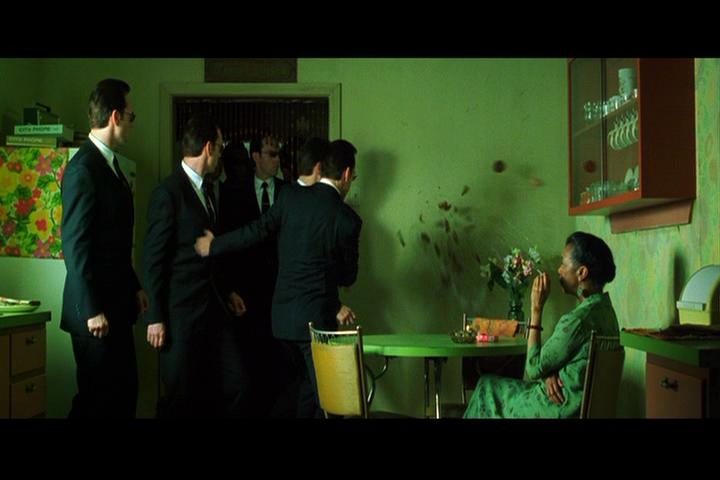
\includegraphics[width=0.5\linewidth]{fig/45c00df489aee5ef7609d702.jpg}
\end{figure}

\myparsep

\begin{myquote}
Roland: I want the truth. I don't care what it takes. Make him remember.

Mauser: Sir? We found her!

Roland: The Logos?

Mauser: Yes, sir.

Roland: 'Bout time we had some god damn good news.

Morpheus: Are the thermals picking up any signs of life?

AK: No, sir. Nothing yet.

Roland: What about the ship?

AK: Well, holographic says the hull is still intact.

Roland: Drop her down [...]

Colt: Yes, sir.

Roland: Get a full diagnostic on that ship as fast as humanly possible.
\end{myquote}

这里Roland在说“好消息”的时候又用了god damn一词,就是说这个“好消息”也是注定的。这里挺有意思的是,老莫很着急地问“有生命信号吗?”听到否定的回答,就一脸伤心样。当然了,他担心的是Niobe。至于Ghost和Sparks, 老莫只会来一句“他们都是好同志”。

\begin{myquote}
Colt: Careful, sir! The squids are sneaky bastards. Could be a trap.

AK: What was that?

Niobe: You can put that shit away, boys. All she needs is a jump.

Morpheus: Niobe.

Niobe: Morpheus. Are you all right?

Morpheus: Yes, I'm fine. We didn't know what happened after. I'm sorry.

Niobe: It's okay. I'm happy to see you too. Did you get Neo out?

Morpheus: Yes. How did you know about that?

Niobe: The Oracle.

Morpheus: You saw her?

Niobe: Just before the sentinels found us.

Morpheus: What did she tell you?

Niobe: The same thing she always does. Exactly what I needed to hear.
\end{myquote}

先知总对Niobe说的就是那句“你自己拿主意”。Niobe说这是自己正想听的,正好突出Niobe果断的性格。Don Davis为Niobe开飞船所做的配乐名叫Die Brünett Walküre,是德文的,这个名字来自尼采最喜欢的一位德国作曲家瓦格纳的作品,Der Ring des Nibelungen(尼伯龙根的指环),其中第二部分就叫做Die Walküre(女武神)。而Brünett意思是棕色头发,Niobe就是棕色头发的女武神。

\begin{myquote}
Lock: In less than 12 hours, the machines will breach the dock walls. Every simulation we've run, we've seen that once the machines are inside the city, the odds of our survival decrease dramatically. Thus our primary objective must be to destroy or disable the diggers inside the dock. If we can do that, perhaps we can prevent them from ever reaching the city. If not, the only place we'll be able to mount an effective defense will be at the entrance of the Temple. It is small enough that it will force them into a bottleneck, allowing us to concentrate the remainder of our defense.

Councillor Dillard: We understand that you've requested additional volunteers.

Lock: That is correct.

Councillor West: Precisely what size of force are you planning to commit to the primary dock objective?

Lock: Right now, the entire APU core and half the infantry.

Councillor West: Half the infantry?

Lock: If it were up to me, Councillor, I'd take every man, woman, and child, put a gun in their hands and march them straight into that dock.

Councillor Dillard: Perhaps it is best that it is not up to you.

Lock: Time will tell, Councillor.

Councillor Hamann: Commander, just one more question. Has there been word from the Nebuchadnezzar?

Lock: None, and at this point there's no reason to expect that there ever will be.

Councillor Hamann: Perhaps. But we can hope.

Lock: I'm afraid hope is an indulgence I don't have time for.
\end{myquote}

黑客帝国的思想分为三部分,Zion是身体,Matrix是思想,Machine是灵魂。在真实世界很少有很高深的内容,就解释一下这些人名字的含义吧。

议会成员:

Councillor Hamann指的是Johann Georg Hamann,是个德国哲学家,也是康德的好朋友。齐泽克就曾指出导演兄弟一定非常了解康德。虽然导演也很了解哈曼,但是并不相信他的很多东西。有趣的是,康德影响了叔本华,哈曼影响了黑格尔,叔本华和黑格尔却又是死对头,站在叔本华这边的导演当然不会过多地加入哈曼的东西。比如他在第二部和Neo讨论什么是控制的时候,只涉及了“定义”的问题,这类似黑格尔的感性确定性,是很小一部分导演认为黑格尔说对的东西。

Councillor Dillard指的是作家Annie Dillard,她曾获1975年的普利策奖。导演用这个名字就是因为喜欢她的诗歌而已。既然不是哲学家,我也就没什么说的了。

Councillor West指的是哲学家Cornel West,他的扮演者就是Cornel West本人。他是导演的私人朋友,但在电影里并没有明确指出他的理论,那说一些有趣的事吧。这个家伙在做黑客帝国评论音轨的时候老是抢着说话,我记得郭大路兄的《终结套装观碟笔记》里说他对东方哲学还有佛学很有研究。这就是我觉得他有意思的地方,因为和他一起做音轨的“心理学的爱因斯坦”Ken Wilber更厉害,Ken曾经在西藏跟六个大仁波切学禅,比West正规得多,而West却总是抢着说佛教方面的东西。

\begin{myquote}
Cas: Zee, what are you doing?

Zee: Making shells.

Cas: They're evacuating our level. We have to go.

Zee: I'm not going with you.

Cas: What?

Zee: They've called for volunteers to hold the dock.

Cas: *to the kids* Kids, you stay here. *to Zee* I know how you feel, Zee, but you can't do that.

Zee: I have to.

Cas: Why?

Zee: Because I love him. I love him the same as he loves me. And if I were out there and he were here, I know [what he'd do].

Cas: But you're gonna get yourself killed. It's crazy, Zee.

Zee: Maybe it is. But ask yourself, if it were Dozer, and you knew the only chance you had to see him again was to hold the dock, what would you do?

Cas: Make shells.
\end{myquote}

简单的对话,无非是表现“爱”这个大多数哲学家不以为然的东西,但用在这里却挺合适的。Matrix里的人都是深沉的、哲学的,Zion里的人都是热情的、情绪化的。所以说,写到这里就是我最头痛的部分了。

\begin{myquote}
Mifune: What the shit is going on over here?

Kid: An accident, sir! I didn't see ... I'm sorry!

Mifune: Who the hell are you?

Kid: I'm here to volunteer, sir.

Mifune: What's a pod-born pencil-neck like you doin' volunteering for my corps?

Kid: I want to do my part, sir! We gotta hold the dock.

Mifune: How old are you, kid?

Kid: Eighteen.

Mifune: Shoulda said sixteen, I mighta believed that!

Kid: OK, I'm sixteen.

Mifune: Minimal age for the corps is eighteen. Sixteen's too young!

Kid: The machines won't care how old I am. They'll kill me just the same.

Mifune: Ain't that the god damned truth?

Kid: Give me a chance, sir. I won't let you down.

Mifune: You do ... you'll find me and the machines have something in common.
\end{myquote}

解释一下Kid的名字,他其实就是黑客帝国动画版中Kid's Story中的那个小子。他在Matrix中的名字是Michael Karl Popper,暗指一个奥地利哲学家Karl Raimund Popper。他最著名的理论就是对观测归纳法的批判,Kid正是通过质疑观测归纳法脱离Matrix的。而那个名字Michael就不确定了,一来导演俩是乔丹迷,可能用了他的名字;二来也可能指炽天使米迦勒(St. Michael)。我个人倾向于米迦勒的解释,因为导演在解释Morpheus眼镜反射Neo选药片的镜头时说过,右边镜片里是Neo和红药片,左边的代表Anderson先生和蓝药片。那么说明导演为这个Kid也准备了两种身份,Matrix中那个应该对应米迦勒的反面,熟悉圣经的朋友应该知道,米迦勒的双胞胎兄弟就是堕天使Satan,而Kid也正是从楼上跳下来摔死的。另外,TomCatMao兄指出过Kid在学校的Locker上画着一条向下冲的龙,代表Kid将跳楼而死。而Satan堕天的时候正是以龙型降世,尾巴扫下天上三分之一的星。

\begin{myquote}
Ghost (v. o.): Okay. Charge the igniter.

Sparks: She lives again.

AK: You want us to patch an uplink to reload the operations software, Sparky?

Sparks: Yeah, that'd be swell. You can clean the windshield while you're at it. Uplinks are in place. I'm bringing her back online. Looking good, except, uh ... something wrong with the Matrix feed.

AK: No, there's not. You're looking at what we're looking at.

Sparks (v. o.): What the hell's going on in there?

Link: Whatever it is, it can't be good.
\end{myquote}

这里的问题我在前面说过了,是Smith的蔓延影响了系统的信号。这里还要强调的是黑暗的含义,先知说的“我看见黑暗在蔓延”指的就是Smith的黑暗。前文中我引用了一个拉丁文谚语“智慧的神用黑暗卷起未来”,现在就具体解释这是什么样的黑暗。印度教经典《奥义书》的基础篇《依沙奥义书》第12句为“沉迷于大千世界者堕入黑暗,致力于不可见神力者进入更大的黑暗”,这两个黑暗就有本质的不同,前者就如Smith的那种黑暗,沉迷于表象;后者就如涅槃,进入全知全能、绝对自由的世界。Smith的黑暗来自于他的地位,也就是前面提到过的“大他者”,那个只能维持自身的可怜虫。他的黑暗其实是智慧的,他完全可以算是一个智慧的神,他也曾经多次把自己比作为上帝。比如在ETM游戏中,Niobe和Ghost遇到他的时候,他说:“I'm the alpha of your omega, the beginning of your end.”这是按照圣经的启示录1:8:“I'm the alpha, I'm the omega, I'm the beginning, I'm the end.”(各版本有所不同)说的。如果说Smith最后胜利了,那未来一样是智慧的,只是这智慧属于Smith一人,属于大他者本身,所以无论人还是机器都视他为最大的敌人。

话说回来,被Smith入侵算不算是涅槃呢?Smith既然是大他者,就是宇宙的本体,你加入了Smith就等于“和宇宙灵魂合为一体”。但是你还没有得到梵,没有获得真知,那将是更深一层的摩耶,更难脱离的轮回。

\begin{figure}[htb]
\centering
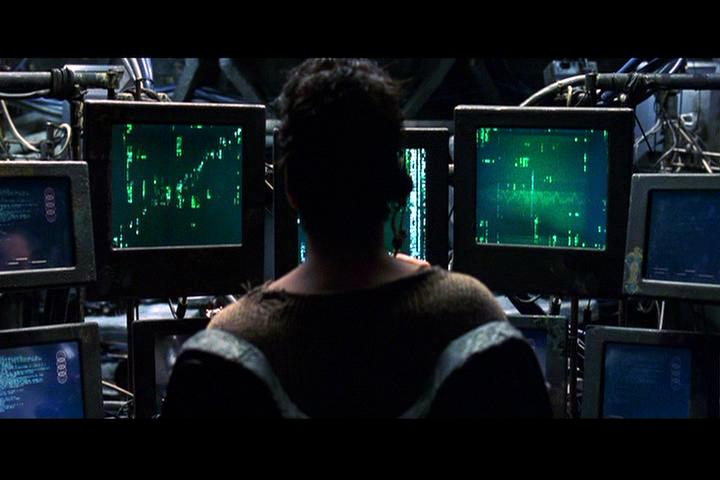
\includegraphics[width=0.5\linewidth]{fig/e7e946101bf652fcc2ce7923.jpg}
\end{figure}

\begin{myquote}
Roland: The machines have taken Junction 21. The way I see it, if we drop down from broadcast here, at Interstate 153, we might surprise them. We go first, hammer as deep as we can, them blow our EMP. Hopefully, we can punch a hole big enough for you to get through.

Niobe: *sighs*

Roland: It ain't pretty, but the way I see it, it's the only way back.

Niobe: No it's not. There's another way. A support line. It drops down right here. A thousand meters short of 21. If we're lucky, we may be able to slip down without them ever knowing.

Roland: That's a mechanical line. It's impossible. No one can pilot mechanical.

Niobe: I can.

Roland: Bullshit.

Niobe: I've done it.

Morpheus: That was a long time ago, Niobe.

Niobe: I said I can do it.

Roland: So what? If you can, you'll be the only one that can. There's no way we can follow you.

Neo: Hi. I know time is always against us, and I'm sorry I took so long. But I wanted to be sure.

Trinity: Sure of what?

Neo: I know what I have to do.

Morpheus: What?

Neo: There's no easy way to say this, so I'll just say it. I have to take one of the ships.

Roland: What?

Morpheus: To go where?

Neo: To the machine city.

Roland: *laughs*

Neo: I know it's difficult to understand ...

Roland: No, it's not --- you're out of your god damn mind.
\end{myquote}

God damn一词又出现了,说明Neo要上机器城完全是预料之中的。谁的预料之中呢?当然是先知。

\begin{myquote}
Neo: I still have to go.

Roland: You'll never make it. Hundred years no ship has gone within a hundred kilometers of it. You'll never make it.

Neo: I have to try.

Morpheus: Is this what the Oracle told you?
\end{myquote}

老莫的反应也很有趣,他一向是信仰先知的,即便在影片的开始他质问过先知。但是到了关键时刻,他还是要问一下是不是先知的计划。

\begin{myquote}
Neo: No.

Roland: This is asinine! If you want to kill yourself, go do it, but do it without wasting one of our ships.

Neo: You have to believe me. I have to go.

Roland: Bullshit! While I'm captain of this ship, I say where it has to go. Believe me, this ship will go to hell long before I let you take it anywhere.
\end{myquote}

“这艘船下地狱”很有趣。neverwin和郭大路都把Zion保卫战称作地狱之战,那画面就是炼狱图,而这艘船就是下地狱的那艘。

\begin{myquote}
Niobe: He can take mine.

Roland: You can't do that.

Niobe: Don't even think of trying to tell me what I can or cannot do with my ship after that little speech.

Roland: But for Christ's sake, Niobe ...
\end{myquote}

为了“基督”,这句话也是很有趣的。Neo就是这个救世主的角色,为了Neo, 那不就是把飞船给他?

\begin{myquote}
Niobe: I'll pilot this ship. He can take mine. If we leave inside an hour, we should reach Zion as the machines do. That's as good a plan as any.

Roland: It's a waste. A god damn waste.

Niobe: Two ships, two directions. Sounds like providence, doesn't it, Morpheus?
\end{myquote}

第二部里,Trinity告诉Neo说老莫和Niobe分手是因为老莫去见了先知,这个就是先知告诉老莫的,老莫一定是以为他们两人不同路。

\begin{myquote}
Morpheus: You've never believed in the One.

Niobe: I still don't.

Morpheus: Then why are you doing this?

Niobe: I believe in him.

Neo: Thank you.
\end{myquote}

这里要提一下Niobe名字的另一个不太为人所知的意思。很多人认为Niobe只是个神话人物,其实导演要暗示是Ebion(换一下字母顺序)。这类人不相信耶稣是上帝的儿子,但是相信耶稣确实是个特殊的人。这里Niobe说自己不相信救世主的预言,但是相信Neo的能力。

\myparsep

\begin{myquote}
Trinity: I'm ready.

Neo: Trinity ... There's something I have to say. Something you need to understand. I know I'm supposed to go. But beyond that --- I don't know ...

Trinity: I know. You don't think you're coming back. I knew it the moment you said you had to leave. I could see it in your face, just like you knew the moment you looked at me that I was coming with you.

Neo: I'm scared, Trin.

Trinity: So am I. Took me ten minutes to buckle up one boot. But I'll tell you something. Six hours ago I told the Merovingian that I was ready to give anything and everything for you. Do you know what's changed in the past 6 hours?

Neo: No.

Trinity: Nothing.
\end{myquote}

两人准备慷慨赴死,没有什么需要详细讲的。不过就是这里让很多人认为Trinity和Merovingian谈判那一段被删了些内容。其实很好理解,Trinity的意思就是“我对他说我愿意为你死,现在我还是一样”。而且Trinity和Merovingian谈判后的剪辑其实很不错,很多优秀的电影都用过切除重要片段的手法来为观众提神,不过这样的手法最早是美国漫画常用的手法。

讲讲欧美漫画充实版面吧。美国的漫画人其实和我们脑子里漫画人的概念很不同,他们往往都是很有阅历、很博学的,不是那种只会画两笔的小青年。特别是在80年代欧美漫画new wave之后的漫画人,基本上都有极丰富的科学知识,就连早期的《超人》也被他们用科学给解释了,NGC专门为《超人》中的科学制作过纪录片。而且他们还都是符号学的专家,不是鲍德里亚那种,而是具体使用的专家。他们放在漫画中的隐喻是很深的,不像是日本漫画总给你拿出来讲。另外还有很多人在专门知识领域里很有研究,最主要的几个领域是政治、科学、医学,像是导演(以前是写漫画的)这样的哲学类也有一些。我知道的少数几个哲学类漫画人现在都在导演门下,比如说Kaare Andrews,他为黑客帝国的漫画系列写了一个关于Kid的故事,名叫I Kant。光这个名字就很有意思,本意是“我做不到”(I can't),改了一下拼写就成了康德(Immanuel Kant)名字的缩写。要知道我在这里一直提的叔本华就受了康德很大的影响,据说他的书桌上就放着康德的画像,Kaare往故事里融合康德哲学很能说明他的哲学底子。而另一位Dave Gibbons的《Butterfly》还引用了老子的《道德经》,居然是直接引用中文的,真不知道有多少欧美漫迷看得明白,估计他们都根据那意境往佛教上理解了。

\begin{myquote}
Roland (v. o.): Are you finished loading that amunition?

Mauser: Just about, sir!

Roland: Let's move it, we are out of time.

Niobe: You're not leaving them anything?

Roland: Said he didn't need it.
\end{myquote}

看来Neo去机器城这个决定是做得很艰难的。一来他知道自己非去不可,二来他知道常规武器没有用。这时候的Neo就和面对Smith的先知一样,只能hope。

\begin{myquote}
Link: *hugs Trinity* I ain't saying goodbye. I'm saying good luck.

Trinity: Thank you.

Morpheus: I can only hope you know what you're doing.

Neo: Me, too. It was an honour, sir.

Morpheus: No, the honour's still mine.
\end{myquote}

在哲学家那条音轨里,Ken和West说这时候的Morpheus终于是个真真正正有血有肉的正常人了。第一部里的Morpheus是神,他告诉我们现实;第二部里的Morpheus是父,他带给我们希望;第三部里的Morpheus是人,为了自己的选择而战斗。老莫在这里的说的honour才是真正被我们感知的那个honour。第一部里戴着反光的墨镜,露出捉摸不透的笑容,那时候哪里有观众感受这个词啊,都在猜老莫是个什么人呢。这里的honour才是一个战士嘴里的honour。

\begin{myquote}
Mauser (v. o.): We're ready, sir.

Roland: 'Bout damn time. *to Niobe* We're already late, captain, so let's hit it and hit it hard.

Niobe: Bye, baby. Take good care of them.
\end{myquote}

女武神要出发了,Logos也要去机器城了。先知的这个预言拆散了老莫和Niobe,但是好在有些事是不会变的。

\begin{figure}[htb]
\centering
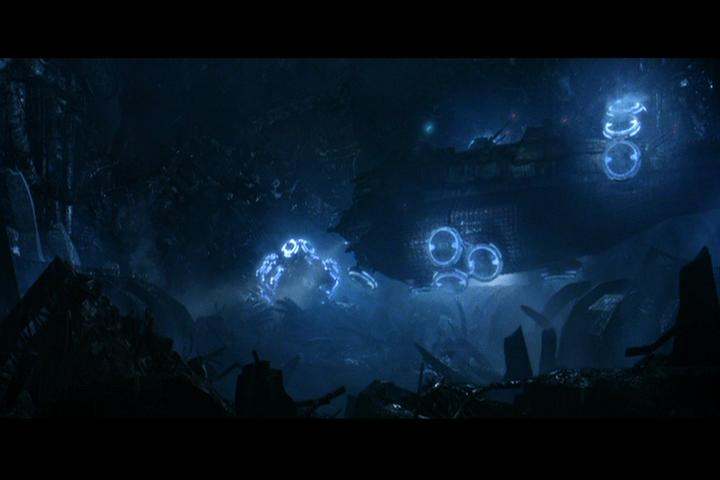
\includegraphics[width=0.5\linewidth]{fig/0c47bd3135fd92a85fdf0e64.jpg}
\end{figure}

\begin{myquote}
Trinity: Ready?

*Neo nods. Trinity punches a button and the lights go out*

Trinity: Engine's still firing. Must be a fuse. I'll check it out.

Bane: I should've known he'd sent his bitch first.

Trinity: Bane?!

Bane: No one ever got away from me as many times as you did. Every single time I thought it was the last. Every time I was sure we had you, but somehow you'd slip through our fingers. I really can't express just how aggravating that can be.

Trinity: What are you talking about?

Bane: I think I might enjoy killing you as much as killing him.

Trinity: Neo! It's Bane, he's psychotic!

Bane: You're gonna pay for that.
\end{myquote}

这个Bane的本意是毒药、祸害,应该不用解释意思了吧。很快我们就要看到黑客帝国三部曲中最真实的打斗了。

\begin{myquote}
Ghost: Twenty-seven kilometers to go.

AK (v. o.): Captain, we've got an emergency down here.

Roland: What is it, AK?

AK: It's Maggie, sir. She's dead. Murdered. I think it was Bane.

Roland: God damn it.
\end{myquote}

又是god damn it, 又是注定的。但是话说回来,什么不是注定的呢?

\begin{myquote}
Roland: I knew it. I knew he was out of his god damn mind. He fired that EMP. God damn it, I should have beaten it out of him.
\end{myquote}

这里的out of mind也很有意思。Smith的mind本来就是在Matrix中,现在溢出到人体里,字面上理解也是out of mind。

\begin{myquote}
Colt: We've searched the whole ship, captain. He ain't here.

Roland: I know where he is.

Morpheus: The Logos.

Link: We gotta go back!

Roland: Too late.

Link: You don't know that. What if they need our help?

Roland: It's too dangerous.

Link: Why?

Morpheus: Because if he's killed them, he'll control another EMP.

Roland: At this point, they're on their own ... just like us.

Bane: Mr.~Anderson. I see you're as predictable in this world as you are in the other.
\end{myquote}

在《黑客帝国》里,说一个人容易预料可以算是最大的侮辱。但事实上,Neo确实很容易被预料,因为Smith理解他和Neo的使命。第一部里Smith还是个特工的时候就很好地预料到了Neo的行踪,在Jones和Brown在下面追赶Neo的时候,Smith就已经在303房间等候他了。

\begin{myquote}
Neo: What?

Trinity: He's out of his mind.
\end{myquote}

这句out of mind又出现了。一语双关的例子在第一部Neo挨老板骂的时候就已经发挥到了极致。这里要纠正一点(也不算是纠正啦,提一下),我在补充Neptuneneo的第一部解读的时候说他老板Rheinheart的名字是来自一位康德派的哲学家,曾经出现在黑格尔的《大逻辑》中;而这个名字现在有了新的解释,这个名字可能来自瓦格纳的歌剧Das Rheingold。因为第三部中有四首配乐的名字对应瓦格纳的《Der Ring des Nibelungen》(尼伯龙根的指环),Das Rheingold正是其中之一。此外,这里的配乐就叫做Das Banegold。

\begin{myquote}
Bane: It might appear that way to you, but Mr.~Anderson and I know that appearances can be deceiving. Confused, Mr.~Anderson? It'll all become clear in a moment. Now, thank you for bringing me the gun. You can set it down right there.
\end{myquote}

这段话第一句是很重要的,黑客帝国官方网站上有一整篇文章就是讲的“对你来说,对我来说”的问题,那位教授用这一点分析了Matrix内外的真实性。而在这里,意思就是个体和对象的转换造成概念指向的差别。

而这里的“appearances can be deceiving”已经成了我一位文学老师的课程之一,关于这一点就不用多说了。笛卡尔的恶魔论、莱布尼兹的单子论、鲍德里亚的后现代、黑格尔的感性确定性、叔本华的表象世界,还有印度教佛教的maya(摩耶)、samsara(轮回)、圣经传道书的空虚为本等等都指出“表象的欺骗性”,也有说表象的作用是“藏起其实不存在的事实”。

\begin{myquote}
Trinity: Don't do it. Shoot. Shoot now.

Bane: Yes, shoot, fry us, burn us alive!

Trinity: Shoot, Neo. If you don't, he'll kill us both.

Bane: Look at him. He knows he should do it but he won't. He can't.

Trinity: Do it.

*Neo puts the gun down*

Bane: Back away from the gun and turn around.

Neo: Let her go.

Bane: Somehow familiar, isn't it? We've been here before, you and I. Remember? I do. I think of nothing else.
\end{myquote}

这里Smith说的就是在第一部里杀死Neo的情形。前面已经提到过了,Smith再生之后一直想的就是复仇。

\begin{myquote}
Neo: Who are you?

Bane: Still don't recognize me? I admit, it is difficult to think, encased in this rotting piece of meat. The stink of it filling every breath, a suffocating cloud you can't escape. *spits blood* Disgusting! Look at how pathetically fragile it is. Nothing this weak is meant to survive.
\end{myquote}

又和第一部呼应了,Smith在审问老莫的时候就说过他讨厌人类的味道,又开始谈论人类不该存在的理论了。

然而,我觉得现在是时候解答neverwin在第二部解释中留下的一个思考题了:法国人看到Neo流血后说的‘看,他只是个人’是什么意思?

这个问题应该和Smith在自己手上划伤痕联系起来解释。圣经中,彼拉多把耶稣交给犹太人时说了Ecce Homo,也就是“看这个人”。这句话有两种意思,一是“看啊,这就是那个人”,这个用法被尼采采用,写下了《Ecce Homo》一书;另一种用法是“看啊,他还是个人”,在耶稣受刑的时候,人们看到创造奇迹的耶稣也会受难,所以说他还是个人。

法国人看到Neo流血而说的“看啊,他还只是个人”就是Ecce Homo的第二种用法,当然也暗示他是救世主。而Smith也一样,他刚刚进入Bane的身体要适应“自己是人”,感受痛苦就是他感觉自己是人的方法。当然了,他还是向往变成神更多一点。

而Ecce Homo的第一种用法也在电影中使用了。配乐大师Don Davis曾经说到过Neo和Smith大战时的配乐,尼采的《Ecce Homo》是一个候选,后来因为效果问题才最终选择了《奥义书》。(《神曲》原本也是个选择)

\begin{myquote}
Neo: What do you want?

Bane: I want what you want.

*Neo looks up with recognition in his eyes*

Bane: Yes ... That's it, Mr.~Anderson. Look past the flesh, look through the soft gelatin of these dull cow eyes and see your enemy.

Neo: No.

Bane: Oh, yes, Mr.~Anderson.

Neo: It can't be.

Bane: There's nowhere I can't go. There's nowhere I won't find you.

Neo: It's impossible.

Bane: Not impossible. Inevitable. Goodbye, Mr.~Anderson.
\end{myquote}

“不可能”和“必然”的问题又出现了,“不可能”的本质就是按过去经验对未来预测的准确度极低,而“必然”的本质就是因果律所指出的。再给一个拉丁谚语吧:Certum est, quia impossibile(这是必然的,因为这不可能)。这在第一部也提到过了,Trinity对Neo说从没有人能这样从特工手中救出人,Neo说:“所以这是可行的。”

\begin{myquote}
Trinity: This is it, it's gotta be. *She pushes a circuit breaker, the lights go out*

*Bane/Neo fight*

Neo: *screams*

Trinity: Oh, no.

Bane: I wish you could see yourself, Mr.~Anderson. The blind messiah. You're a symbol for all of your kind, Mr.~Anderson. Helpless, pathetic. Just waiting to be put out of your misery.
\end{myquote}

这里有个明显的隐喻 --- 弥赛亚,和大喊“Jesus Christ”的用法没多大差别,唯一的小区别就是犹太人恨耶稣,但是企盼弥赛亚的到来。Smith这么一说,就是把不完整的救世主给说完整了。Neo不再只是人类的救世主,而是Matrix和人类共同的救世主。

\begin{myquote}
Neo: I can see you.

Bane: It's not over, Mr.~Anderson. It's not over.

Neo: Trinity!

Trinity: Neo. Oh, no. Your eyes.

Neo: I'll be okay. It's all right, Trin. But I think you're gonna have to drive.
\end{myquote}

\begin{figure}[htb]
\centering
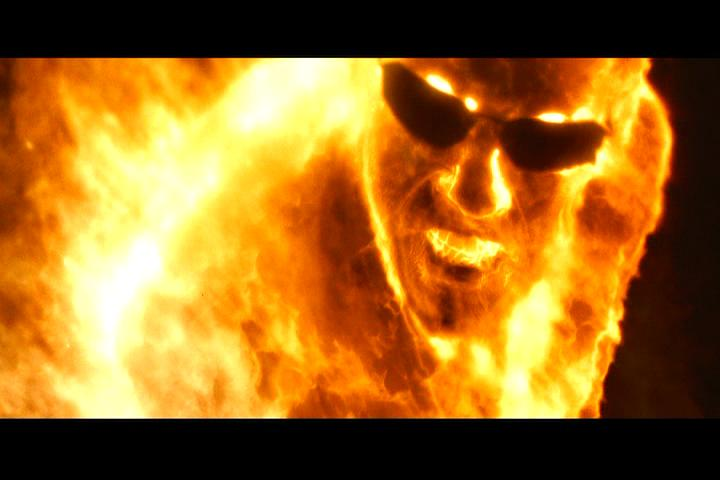
\includegraphics[width=0.5\linewidth]{fig/f64563d00ca0378fa1ec9c63.jpg}
\end{figure}

这个金色的Smith以及后面的金色机器可以算是黑客帝国中最难理解的。这个难不是因为理论的深,而是因为这里不科学。事实上,这里是黑客帝国三部曲最纯粹的哲学表现,不带有丝毫的杂物(呵呵呵,不是说我自己)。鲍德里亚曾经批评《黑客帝国》对他的理论有误解,拟仿物和拟像的关系并不是显而易见的,并不是可以概念化的。鲍德里亚说这件事的时候,只有第一部上映了,所以说鲍德里亚很自然地认为Zion和Matrix是拟仿物和拟像的关系,电影中二者却被清晰地赋予了概念,这就是他觉得“误解”的地方。事实上,真正的拟仿物根本没有在第一部电影中出现。

而分析哲学家,和鲍德里亚代表的后现代主义者一直处于对立位置的那些,按他们自己的分析法来指出《黑客帝国》很好地代表了哲学的后现代主义(他们说其中传统哲学比后现代更为优秀),并批评鲍德里亚用词晦涩难懂,似是而非地回答问题等等缺点,说他们说话的方式比他们说的话更重要。

我个人觉得鲍德里亚的难懂是很正常的,既然拟仿物和拟像的关系非常不明确,或者如其他理论说的拟仿物根本不存在,鲍德里亚若是使用十分清晰的字眼就更容易出现读者的误读,倒是导演这种视觉做法很容易解释哲学的后现代。

这个金色的Smith才是三部曲中唯一的拟仿物。既然拟仿物是超越我们感官的,那么我们就看不见这些东西。而导演安排Neo在眼瞎之后看到真正的拟仿物,很明显是告诉我们这个金色的Smith是个表现形,是超越我们视力的。叔本华说过我们视野中的任何东西都不能证明我们是在用眼睛看,这就是允许这个逻辑矛盾存在的依据。

我们黑迷在谈到金色光芒的时候,习惯管这叫精神、灵魂,我认为这更像是莱布尼兹所说的“单子”,或者是黑格尔感性确定性中那个不存在的“完美概念”,也可以是柏拉图洞穴寓言中无限真实的“Good”,也可以是印度教中的“涅槃”,也可以是《传道书》中说的空虚,也可以是真实的缺失的表现。但是,我们看到的画面又绝对和我上面提到的这些理论不一致,因为这是不能被概念化的。任何一种对金色光芒的解释都是错误的,我们唯一能做的就是给它取个名字,不能叫“灵魂”,因为灵魂和莱布尼兹的“单子”太接近了;不能叫“意志”,意志极抽象,但是富于概念性;应该叫“精神”,因为精神的概念是很模糊的,机器的精神就更为模糊了。如果叫做“灵魂”的话,就肤浅了,因为那会被理解为机器的信息层面;如果叫“意志”,那就偏差了,因为那会被理解为机器的自主目的。所以“精神”是迄今为止最好的叫法。当然,最好的表现法仍然是电影中直接的表现法,把机器的“精神”嵌入逻辑的矛盾(瞎眼的视野)中,致使我们无法定义它,又让观众有了个直观的感受。

除了电影中的做法,任何其他对拟仿物的描述都是偏差的、肤浅的。“机器的灵魂”是肤浅的,“机器的意志”是偏差的,“机器的思维”是狭隘的。《黑客帝国3》对模仿和拟像的描述是不可超越的,就连鲍德里亚本人也不能超越《黑客帝国3》,因为他仍然用文字,他仍然使用定义归纳。《黑客帝国3》不仅是后现代拟像描述的典范,还是后现代拟像描述的极至!难怪那个分析哲学家Richard Hanley说如果他也拍电影解释的话,根本不会把鲍德里亚放在眼里。

但讽刺的是,这种极至的哲学看上去和哲学没有多大关系,要接近理解(完全理解是不允许的)它需要绕一个哲学的大弯才行。

\myparsep

\begin{myquote}
Lock's Lieutenant: Seismic's projecting twenty-two minutes to breach.

Lock: They can't know we don't have an EMP, they'll have to attack in waves. Concentrate our offense on the diggers. Order the APUs into position.

Lock's Lieutenant: Yes, sir.
\end{myquote}

最高指挥官Jason Lock和老莫是情敌,估计是他和Niobe一样不相信救世主才走到一起的。所以说当Niobe说他相信Neo的时候,也是Niobe和Lock划清界限的时候。

根据Matrix Dictionary的说法,他是唯一一个有全名的Zion人员。这个家伙是个hardass, 很多船员都管他叫deadbolt(主要是Logos的接线员Sparks这么叫他)。这个外号和他的名字其实很相配,lock是锁的意思,bolt是门闩的意思。作为Zion的指挥官,他的任务就是锁住Zion的大门。

另外,Lock也是暗示一个英国的哲学家John Locke。他虽然不是自然哲学家、形而上学家,但也研究认识论,和伯克利等人被归类为经验论者,这点对黑迷来说应该不会陌生,我翻译的《哲学家探索黑客帝国》一书中就有关于伯克利哲学和《黑客帝国》的文章。总的来说Locke是个很务实的人,指挥官Lock也一样。

而他的名字Jason则是一个希腊神话中的英雄的名字,伊阿宋。呵呵,不知道怎么出现的这个音译,可能古希腊语的发音和西班牙语很接近吧(J都是发Y的音)。

\begin{figure}[htb]
\centering
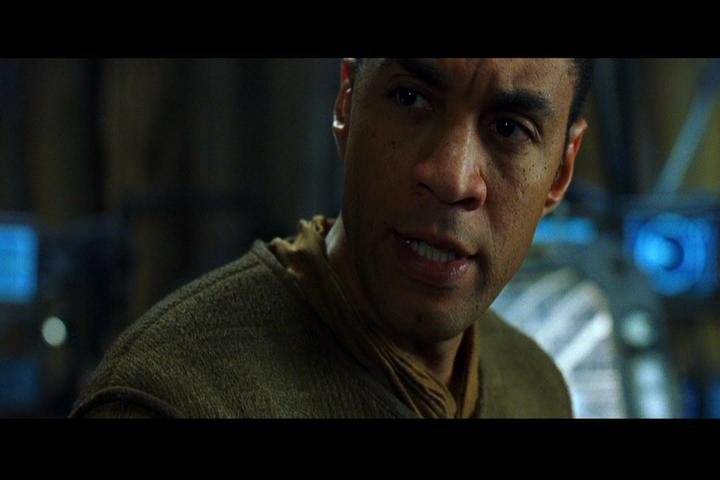
\includegraphics[width=0.5\linewidth]{fig/5fe264383ee43a2397ddd8f2.jpg}
\end{figure}

\begin{myquote}
Mifune: All right, this is it. Now, you all know me, so I'll just say this as simple as I can. If it's our time to die, it's our time. All I ask is: if we have to give these bastards our lives, we give 'em hell before we do!

APU fighters: *cheer*
\end{myquote}

这个APU的意思是Armored Personnel Units,据说这个设计在现实中也有很高的可行性。而Mifune这段战前宣言也够简短的,但是很有气势。导演俩拍电影废话没有一句,该说的就说,不该说的就不说。这样的结果是很有趣的,比如那些哲学探讨,看电影不带脑子的人看着就惨了,一大段一大段的东西根本消化不了,而正好研究这种理论的哲学家们就对这些谈话感到无聊了。(还好《黑客帝国》不是我拍的,我得把每样东西讲得格外清楚才罢手,估计没几个人受得了)

\begin{figure}[htb]
\centering
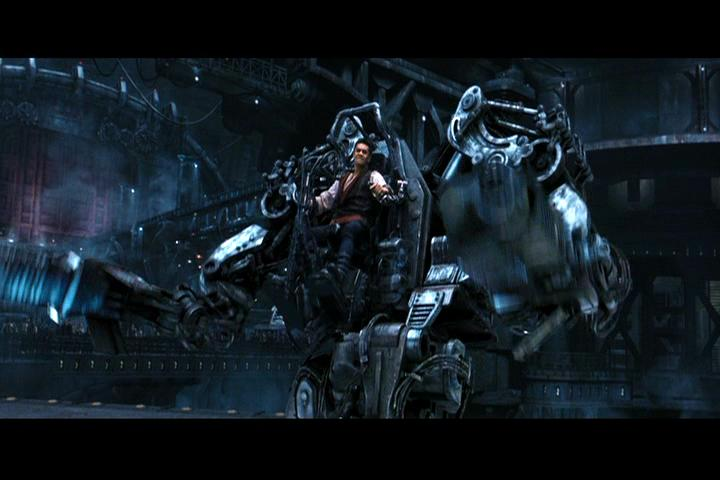
\includegraphics[width=0.5\linewidth]{fig/385658828a847ba20cf4d2f2.jpg}
\end{figure}

\begin{myquote}
Zee: You scared, Charra?

Charra: Shit, yeah. I'll make you a deal, though. You keep loadin', I keep shootin'.

Zee: Deal.
\end{myquote}

接线员Link的老婆Zee加入了Lock征求的志愿者,和她一组的Charra名字是西班牙语女牛仔的意思。

这一段从Lock开始到Zee这里的一段戏描写的就是Zion的各个阶层对Zion大战的准备。这个被neverwin和郭大路称为末日之战的大战中,也是有很多隐喻的,不过哲学内容少了,所以Ken和West在制作音轨的时候没有对这里进行多少评论。我在这里主要也就是挖些隐喻出来。

\begin{figure}[htb]
\centering
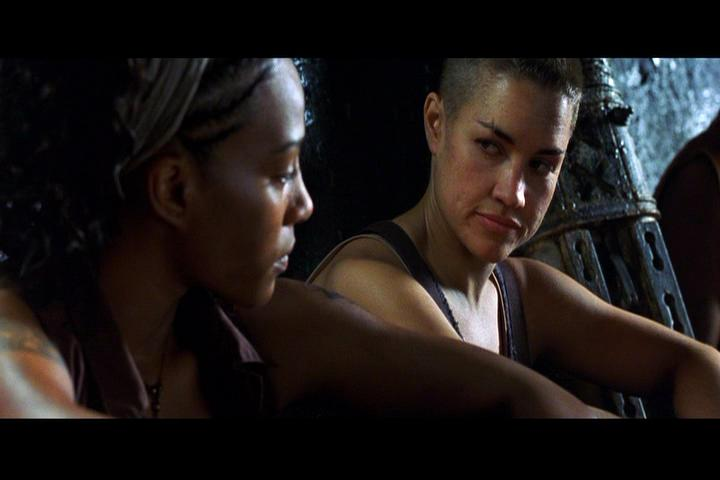
\includegraphics[width=0.5\linewidth]{fig/27d5d1a236c79aadcbefd0f2.jpg}
\end{figure}

\begin{myquote}
AK: Holy Christ. Would you look at that?

Roland: Quiet. [How far down?]

Ghost: 1.4 kilometers.

Morpheus: Still generating too hot field.

Niobe: Ghost, kill all auxiliary systems. Give me full manual, drop down to four pads.

AK: It'll bottom out!

Niobe: Easy, baby.

Ghost: 700 meters.

Niobe: If we can just get close enough.

Ghost: 600 meters.

AK: There.

Niobe: Shit!

Ghost: Jig's up, here they come.

Niobe: Give me full power, full systems!

Roland: Man the gun turrets, every goddamn one of 'em!

Niobe: Ghost, you're the best gunner we have, go with them. Morpheus, take his place!

Link: I'm comin', baby.

Morpheus: Here they come.

Roland (v. o.): Slow down, this ain't the Logos!

Niobe: Hold on to your lunch, Roland, here we go.

Roland: Holy Christ! Didn't know this ship could do that.
\end{myquote}

现在他们要做的就是抢时间。Morpheus在第一部就说“时间总是和我们作对”。我在火车站的场景中就说过了,导演对摩耶三限制“空间、时间、因果”的刻画是很注重的。我们在看电影的时候可以注意到,自从Neo第一次进入Matrix,他们总是在和时间赛跑,无论是从先知那里出来躲避特工,在Cypher杀死Neo之前干掉Cypher,还是在老莫招供之前救出他,或是在乌贼杀死他们之前接起303房间的电话。Neb在第二部里36小时的充电也是匆忙的(老莫下船时就叫Link尽快准备),Neo准时去见先知,又必须在12点整见Merovingian,在高速公路上救起就要被火焰吞没的老莫和Keymaker,Trinity要在他们进入大楼前破坏电力设备,Neo要在Trinity坠楼之前接起她,Neb的船员还要快速撤离要被炸毁的飞船。到了第三部,完全就是建立在赛跑上的。

所以老莫说的“always”就是字面上的always!他们就是永远和时间赛跑的人。

赛跑中有些很有趣的细节,比如Link对这条手链的态度改变。根据Link在第二部中和Zee的对话,我们知道他并不相信救世主的说法,他来当接线员是因为他对Dozer发过誓,然而他在看到Neo的能力之后开始相信了。而在Neo和Smith的最终大战之前,他说了一句:“Neo, if you gonna do something, you better do it quick.”他完全把Neo的胜利当作时间问题了。

这和手链的信仰是一模一样的,从开始的“你知道我不信这套的”到第二部的“戴着也无妨”到这里的“宝贝,我回来了”。Link就从Niobe一样的无神论转变到了Morpheus的深度信仰。

\begin{figure}[htb]
\centering
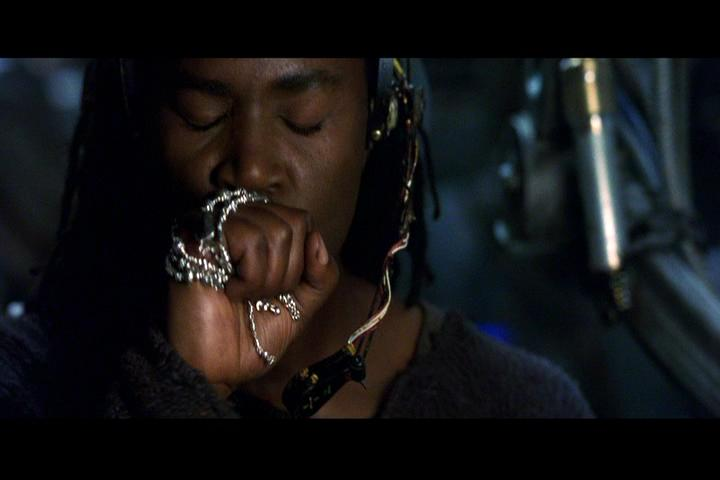
\includegraphics[width=0.5\linewidth]{fig/aea59e3d72117d00bba16754.jpg}
\end{figure}

图片可能不清楚,这里是一个大个头的电子乌贼先出来定位,然后一大群小型的乌贼就冲出来了。在幕后花絮里,工作人员说过他们设计了很多不同种类的电子乌贼,因为导演很注意“目的”,所以就需要很多有不同“目的”的乌贼来打这场仗。其实乌贼的15条触手都有不同的用处。(种类不同,触手数也可能不同,花絮碟里提到的是15个触手的那种)

“目的”可以说是《黑客帝国》最主要的主题,Neo和先知就“目的”的问题大谈过一场。我们常说的“意义”就是目的的一个变体。Sati是因为没有目的而面临删除,Merovingian一帮人因为目的过期而面临删除,Keymaker因为目的完成而被删除,第一部里的特工Jones和Brown因为目的完成失败而被删除。总之,机器的存在是有目的的。而人类呢?虽然尼采批判过consensus sapientium(智者的一致),而且就是对“人生没有意义”的批判,但是大多数哲学家都认为生命是没有目的的(不知道为什么罗素说叔本华是唯一的悲观哲学家)。

按照亚里士多德的原因论,任何事物都有质料因、形式因、动力因和目的因,而他最主要讲的就是目的因中的自然目的论(和意义有很大区别)。他说过:“如果看不见运动者有意图,就不承认有目的因存在,这是荒谬的。”(呵呵,看不到黑客帝国的哲学就说没有,这也是荒谬的)所以人类的存在是有目的的,但这是自然目的,因为人类的诞生并非意识的结果。而像尼采这样赋予人生以目的或是意义,则是人为的目的论,是技术目的,是行为目的。

尽管人类的存在没有意义(我说过我是叔本华派的,你当然可以不同意),但是Neo也有足够理由保护Zion。既然任何存在都没有意义,那么“不存在”也绝无意义可言,那么机器毁灭人类虽然有技术目的,有行为目的,但是并非自然的(即使是进化所需,也不用赶尽杀绝)。

这也就是我在解释Revolutions这个标题时说的关于程序和人类固有目的的革命。

\begin{figure}[htb]
\centering
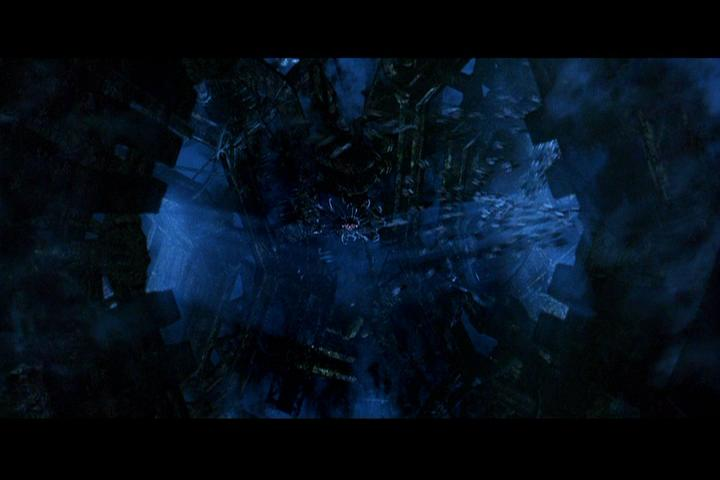
\includegraphics[width=0.5\linewidth]{fig/d272b81259316fcec2fd7854.jpg}
\end{figure}

\begin{myquote}
Operations Officer Mattis: Breached! The dock is breached!
\end{myquote}

首先,这个官员名字,Mattis, 指的是美国海军陆战队一位著名中将James Mattis,研究中东局势、伊拉克战争的人都应该听说过这个名字。

Zion被突破,一个巨大的digger掉下来,这个digger的造型就是倒置着的巴别塔。圣经的创世纪中记载人们想要造一座通天的巨塔,上帝怕人们齐心就可以做到任何事情,所以就使得人们说不同的语言,让人们之间不能交流,结果这座塔就没有建成。巴别塔的作用原本是通天,而在Matrix中,Zion才是真实的世界,是天堂,所以Digger就像是倒置的巴别塔一样挖到Zion。此外,巴别塔的意象在1927年的《大都会》中也出现了。

巴别塔最初的原型被认为是Tower of Jupiter Belus,即巴比伦的米罗达之塔。而有趣的是,建造这座塔的人就是我们所熟知的Nebuchadnezzar,老莫飞船的名字嘛。

\begin{figure}[htb]
\centering
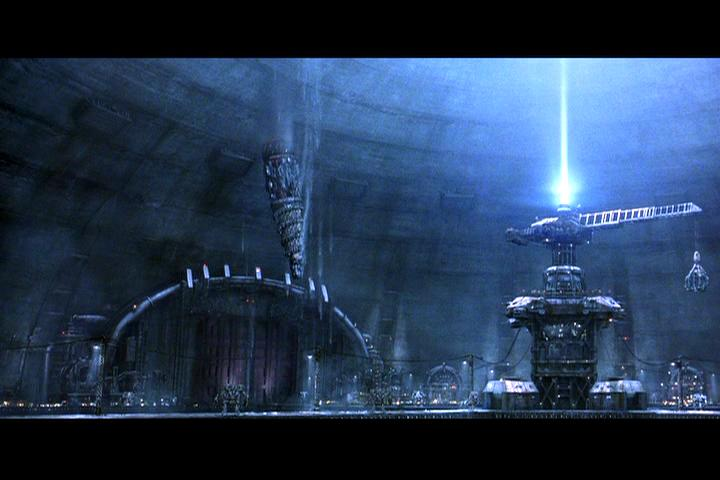
\includegraphics[width=0.5\linewidth]{fig/9f1903089ad2bcd162d986ee.jpg}
\end{figure}

\end{document}
